%%%%%%%%%%%%%%%%%%%%%%%%%
% Dokumentinformationen %
%%%%%%%%%%%%%%%%%%%%%%%%%
\newcommand{\titleinfo}{Partielle Differential Gleichungen}
\newcommand{\authorinfo}{Theory: S. Eicher, Numerik: L. Schmid, S. Eicher, R.
Koller, S. Boller, S. Bischof, D. Strebel}
\newcommand{\versioninfo}{FS2013}

%%%%%%%%%%%%%%%%%%%%%%%%%%%%%%%%%%%%%%%%%%%%%
% Standard projektübergreifender Header für
% - Makros 
% - Farben
% - Mathematische Operatoren 
%
% DORT NUR ERGÄNZEN, NICHTS LÖSCHEN
%%%%%%%%%%%%%%%%%%%%%%%%%%%%%%%%%%%%%%%%%%%%%  
% Genereller Header
\documentclass[10pt,twoside,a4paper,fleqn]{article}
\usepackage[utf8]{inputenc}
\usepackage[left=1cm,right=1cm,top=1cm,bottom=1cm,includeheadfoot]{geometry}
\usepackage[ngerman]{babel,varioref}
\usepackage[T1]{fontenc}

% Pakete
\usepackage{amssymb}
\usepackage{amsmath}
\usepackage{bm} %bold math symbols
\usepackage{fancybox}
\usepackage{graphicx}
\usepackage{color}
\usepackage{xcolor}
\usepackage{lastpage}
\usepackage{wrapfig}
\usepackage{fancyhdr}
\usepackage{hyperref}
\usepackage{verbatim}
\usepackage{floatflt}
\usepackage{arydshln}
\usepackage{ucs}
\usepackage{pdflscape} % landscape
\usepackage{multirow} % zellen in tabellen verbinden
\usepackage{multicol} 
%s\usepackage{diagbox} % getrennte zelle in tabelle
% \usepackage{array} % anordnung in tabellen

%%%%%%%%%%%%%%%%%%%%
% Generelle Makros %
%%%%%%%%%%%%%%%%%%%%
\newcommand{\formelbuch}[1]{$_{\textcolor{red}{\mbox{\small{S#1}}}}$}
\newcommand{\verweis}[2]{ {\small (siehe auch \ref{#1}, #2 (S. \pageref{#1}))
}}
\newcommand{\subsubadd}[1]{\textcolor{black}{\mbox{#1}}}
\newenvironment{liste}[0]{
	\begin{list}{$\bullet$}{\setlength{\itemsep}{0cm}\setlength{\parsep}{0cm} \setlength{\topsep}{0cm}}}
    {\end{list}}
    
\newcommand{\logd}[0]{\log_{10}}
\newcommand{\subsubsubsection}[1]{\textbf{#1}}

\newenvironment{aufzaehlung}[0]{
	\begin{enumerate}{\setlength{\itemsep}{0cm}\setlength{\parsep}{0cm}
	\setlength{\topsep}{0cm}}} {\end{enumerate}}    

\newcommand{\abbHeight}[3]{
	\begin{center}
		\includegraphics[height=#2]{./bilder/#1} \\
		#3
    \end{center}
}

%\newcommand{\skriptsection}[2]{\section{#1 {\tiny Skript S. #2}}}
%\newcommand{\skriptsubsection}[2]{\subsection{#1 {\tiny Skript S. #2}}}
%\newcommand{\skriptsubsubsection}[2]{\subsubsection{#1 {\tiny Skript S. #2}}}
%\renewcommand{\skriptsection}[2]{\section{#1 {\tiny Schaum S. #2}}}
%\renewcommand{\skriptsubsection}[2]{\subsection{#1 {\tiny Schaum S. #2}}}
%\renewcommand{\skriptsubsubsection}[2]{\subsubsection{#1 {\tiny Schaum S. #2}}}
\newcommand{\skriptsection}[2]{\section{#1 \formelbuch{#2}}}
\newcommand{\skriptsubsection}[2]{\subsection{#1 \formelbuch{#2}}}
\newcommand{\skriptsubsubsection}[2]{\subsubsection{#1 \formelbuch{#2}}}

%%%%%%%%%%
% Farben %
%%%%%%%%%%
\definecolor{black}{rgb}{0,0,0}
\definecolor{red}{rgb}{1,0,0}
\definecolor{white}{rgb}{1,1,1}
\definecolor{grey}{rgb}{0.8,0.8,0.8}

%%%%%%%%%%%%%%%%%%%%%%%%%%%%
% Mathematische Operatoren %
%%%%%%%%%%%%%%%%%%%%%%%%%%%%
\DeclareMathOperator{\sinc}{sinc}
\DeclareMathOperator{\sgn}{sgn}
\DeclareMathOperator{\tr}{tr}
\DeclareMathOperator{\tridiag}{tridiag}



% Fouriertransformationen
\unitlength1cm
\newcommand{\FT}
{
\begin{picture}(1,0.5)
\put(0.2,0.1){\circle{0.14}}\put(0.27,0.1){\line(1,0){0.5}}\put(0.77,0.1){\circle*{0.14}}
\end{picture}
}


\newcommand{\IFT}
{
\begin{picture}(1,0.5)
\put(0.2,0.1){\circle*{0.14}}\put(0.27,0.1){\line(1,0){0.45}}\put(0.77,0.1){\circle{0.14}}
\end{picture}
}

\newcommand{\todo}[1]{\colorbox{red}{\textbf{#1}}}
\newcommand{\e}{\mathrm{e}}
\newcommand{\grad}[1]{\underset{#1}{\mathrm{grad~}}}
\DeclareMathOperator{\Real}{Re}
\DeclareMathOperator{\Imag}{Im}

\newcommand{\cfbox}[2]{%
    \colorlet{currentcolor}{.}%
    {\color{#1}%
    \fbox{\color{currentcolor}#2}}%
}


\newcommand{\partFrac}[2]{\frac{\partial #1}{\partial #2}}

%%%%%%%%%%%%%%%%%%%%%%%%%%%%
% Allgemeine Einstellungen %
%%%%%%%%%%%%%%%%%%%%%%%%%%%%
%pdf info
\hypersetup{pdfauthor={\authorinfo},pdftitle={\titleinfo},colorlinks=false}
\author{\authorinfo}
\title{\titleinfo}

%Kopf- und Fusszeile
\pagestyle{fancy}
\fancyhf{}
%Linien oben und unten
\renewcommand{\headrulewidth}{0.5pt} 
\renewcommand{\footrulewidth}{0.5pt}


\fancyhead[L]{\titleinfo{ }- Summary}
%Kopfzeile rechts bzw. aussen
\fancyhead[R]{\today{ }- Page \thepage/\pageref{LastPage}}
\fancyfoot[C]{\copyright{ }\authorinfo}

% Einr�cken verhindern versuchen
\setlength{\parindent}{0pt}



% Möglichst keine Ergänzungen hier, sondern in header.tex
\begin{document} 
 
%%%%%%%%%%%%%%%%%%%%%%%%%%%%%%%%%%%%%%%%%%%%%%%%%%%%%%%%%%%%%%%%%%%%%%%%%%%%%%%%%%%%%%%%%%%%%%%
%%%%%%%%%%%%%%%%%%%%%%%%%%%%%%%%%%%%%%%%%%%%%%%%%%%%%%%%%%%%%%%%%%%%%%%%%%%%%%%%%%%%%%%%%%%%%%%


\section{Theory}

\subsection{Begriffe und Klassifikation}

\subsubsection{Ordnung}

Wie bei gewöhnlichen Differentialgleichungen ist die Ordnung
die höchste Ableitung der unbekannten Funktion, die in der
Differentialgleichung vorkommt.\\

\textbf{PDGL 1.Ordnung: } \qquad$F\biggl(x_1,\dots,x_n, u, \frac{\partial u}{\partial x_1},\dots,\frac{\partial u}{\partial x_n}\biggr)$

Sie kann durch Substitution $\frac{\partial u}{\partial x_i}\to p_i$ durch  $F(x_1,\dots,x_n,u,p_1,\dots,p_n),$
ausgedrückt werden.\\

\textbf{PDGL 2.Ordnung: } \qquad $F\biggl(x_1,\dots,x_n,u,
\frac{\partial u}{\partial x_1},\dots,\frac{\partial u}{\partial x_n},
\frac{\partial^2 u}{\partial x_1^2},\dots,\frac{\partial^2 u}{\partial x_n^2}\biggr)$

Sie kann durch Substitution $\frac{\partial u}{\partial x_i}\to p_i,~\frac{\partial^2 u}{\partial x_i\partial x_j}\to t_{ij}$ durch
$F(x_1,\dots,x_n,u,p_1,\dots,p_n,t_{11},t_{12},\dots,t_{n,n-1},t_{nn})$
ausgedrückt werden.

\subsubsection{Laplace-Operator}
$u(x,y,z)\quad\Rightarrow\quad \Delta u=\frac{\partial^2u}{\partial x^2}+\frac{\partial^2u}{\partial y^2}+\frac{\partial^2u}{\partial z^2}$

\subsubsection{Umwandlung in System niedriger Ordnung}

\begin{tabular}{ll}
Gegeben:& $F\biggl(x,y,u,\frac{\partial u}{\partial x},\frac{\partial u}{\partial y},
\frac{\partial^2 u}{\partial x^2},\frac{\partial^2 u}{\partial x\partial y},
\frac{\partial^2u}{\partial y^2}\biggr)=0.$\\[0.2cm]
Substitution: & $p=\frac{\partial u}{\partial x},\qquad q=\frac{\partial u}{\partial y}$\\[0.2cm]
Für zweite Ableitungen: & $\frac{\partial^2 u}{\partial x^2}=\frac{\partial p}{\partial x},\quad \frac{\partial^2 u}{\partial x\partial y}=\frac{\partial p}{\partial y}=\frac{\partial q}{\partial x},\quad\frac{\partial^2 u}{\partial y^2}=\frac{\partial q}{\partial y}$\\[0.2cm]
Gleichungssystem 1.Ordnung& $p=\frac{\partial u}{\partial x},\quad q=\frac{\partial u}{\partial y},\quad\frac{\partial p}{\partial y}=\frac{\partial q}{\partial x}$
\end{tabular}

\subsubsection{Notationen einer PDGL, Gebiet $\Omega$}
\begin{minipage}{4cm}
	\begin{tabular}{ll}
	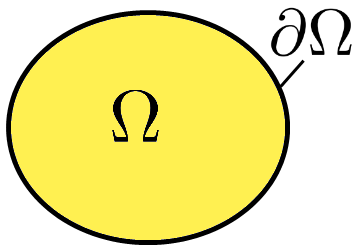
\includegraphics[width=3cm]{Content/Theory/Gebiet}&
	\end{tabular}
\end{minipage}
\begin{minipage}{4cm}	
	\begin{tabular}{ll}
		$\overset{\circ}{\Omega}$ & Innere Punkte\\
		$\partial\Omega$ & Rand\\
		$\overset{\_}{\Omega}$ & Gebiet $\Omega$ und Rand $\partial\Omega$\\
	\end{tabular}
\end{minipage}

Das Gebiet einer PDGL \textbf{muss} offen sein, nur dann ist die partielle Ableitung überall definiert. Das Gebiet ist offen, wenn um jeden Punkt in Gebiet $\Omega$ ein kleiner Ball gezeichnet werden kann, welcher auch in Gebiet $\Omega$ ist.

\textbf{Lösung einer PDGL:}\\
\begin{tabular}{ll}
Gegeben:& Gebiet $\Omega$, PDGL,Randwerte $\partial\Omega$\\
Lösung:& Funktion $u$: $\overset{\_}{\Omega}\rightarrow \mathbb{R}$, PDGL in $\Omega$ und Randwerte auf $\partial\Omega$\\
\end{tabular}

\subsubsection{Klassifikation einer PRGL}


\begin{tabular}{ll}
Ordnung:& Höchste vorkommende partielle Ableitung\\
Type:& Linear:\qquad $F(\ldots)$ lineare Funktion von $u,\frac{\partial u}{\partial x_1},\frac{\partial u}{\partial x_2},\ldots,\frac{\partial u}{\partial x_n}$\\
& Quasilinear: \qquad  $F(\ldots)$ lineare Funktion von $u,\frac{\partial u}{\partial x_1},\frac{\partial u}{\partial x_2},u\frac{\partial u}{\partial x_k},\ldots,\frac{\partial u}{\partial x_n}$, wobei Produkte von \\

\todo{Anschauen}
\end{tabular}

\subsection{Charakteristiken}
\textbf{Wichtig:} Als Anfangsbedingungen dürfen \textbf{keine} Charakteristiken verwendet werden, sonst ist die Charakteristik die Lösung (anstatt Fläche ergibt sich eine Kurve).\\
\textbf{Wichtig:} Die Charakteristik darf den Rand nur einmal durchlaufen.\\
Nützlich für Qasilineare PDGL 1.Ordnung.\todo{Noch mehr?}\\
$$a(x,y,u)\cdot\partFrac{u}{x}+b(x,y,u)\cdot\partFrac{u}{y}=c(x,y,u) \qquad\Rightarrow\qquad a(x,y,u)\cdot\partFrac{u}{x}+b(x,y,u)\cdot\partFrac{u}{y}-c(x,y,u)=0$$\\


\begin{tabular}{ll}
Gebiet:& $\Omega{\ldots|x>0,alle y}$\qquad Randbedingung: $u(0,y_0)=g(y_0)$\\
Vektorielle schreibweise:& $\begin{bmatrix}
	a(x,y,u)\\ b(x,y,u)\\ c(x,y,u)
\end{bmatrix}\cdot 
\underset{\overrightarrow{n}~:~Normale ~auf~ Flaeche}{\underbrace{\begin{bmatrix}
\partFrac{u}{x} & \partFrac{u}{y} & -1
\end{bmatrix}}}=0$\\[1cm]
Tangenten:& $\overrightarrow{t}_x=\begin{bmatrix}1\\0\\ \partFrac{u}{x}\end{bmatrix}\qquad 
			\overrightarrow{t}_y=\begin{bmatrix}0\\1\\ \partFrac{u}{y}\end{bmatrix}$\\[1cm]
Lösungsweg& Für jeden Anfangspunkt $\begin{bmatrix} 0\\y_0\\g(y_0)\end{bmatrix}$ finde eine Charakteristik, diese nach $x$, $y$ auflösen.
\end{tabular}

Beispiel:\\
\begin{enumerate}
	\item PDGL mit Randbedingungen und Definitionsbereich: $\partFrac ux+2\partFrac uy=3$, \; $u(0,y)=g(y)=\sin(y) \Rightarrow u(0,y_0) = g(y_0) = \sin(y_0)$\\
	Therme in Matrixschreibweise: $\begin{bmatrix}a\\b\\c\end{bmatrix}=\begin{bmatrix}1\\2\\3\end{bmatrix}$
	\item Charakteristiken ausrechnen PDGL $\rightarrow$ DGL: 	$\frac {d}{dt}\begin{bmatrix}x(t)\\y(t)\\u(t)\end{bmatrix}=\begin{bmatrix}1\\2\\3\end{bmatrix}$
	\item DGL's lösen (für Standard-DGLS, siehe \ref{sec:dgls} auf Seite \pageref{sec:dgls}.): 
	$\begin{bmatrix}x\\y\\u\end{bmatrix}=\begin{bmatrix}t+x_0\\t+y_0\\t+u_0\end{bmatrix}$
	\item Anfangsbedingungen einsetzen: $\begin{bmatrix}x\\y\\u\end{bmatrix}=\begin{bmatrix}t+x_0\\t+y_0\\t+u_0\end{bmatrix}\Bigg|_{t=0}=
	\begin{bmatrix}x_0\\y_0\\u_0\end{bmatrix}=\begin{bmatrix}0\\y_0\\\sin(y_0)\end{bmatrix}$\\
	Lösung der DGL ist: $\begin{bmatrix}x\\y\\u\end{bmatrix}=\begin{bmatrix}1\\2\\3\end{bmatrix}\cdot t+ \begin{bmatrix}0\\y_0\\\sin(y_0)\end{bmatrix}$\\
	
	\item Eliminieren aller Variablen ausser $u,x,y$: $u=3x+\sin(y-2x)$
	\item Kontrolle
	Resultat ($u=3x+\sin(y-2x)$) ableiten und in Aufgabenstellung einsetzen $\partFrac ux+2\partFrac uy=3$ und schauen ob es erfüllt.
	
\end{enumerate}



\subsection{Methode Separation}
Wahl eines geeigneten Koordinatensystems ist wichtig.


\begin{enumerate}
\item \textbf{Ansatz} (Höchste Ableitung ausschlaggebend): 
	\begin{itemize}
		\item Für PDGL 1.Ordnung: $U(x,y)=X(x) + Y(y)$
		\item Für PDGL 2.Ordnung: $U(x,y)=X(x) \cdot Y(y)$ 
	\end{itemize}
\item \textbf{Einsetzen: } Ansatz in PDGL einsetzen.
\item \textbf{Separation: } Auf jeder Seite der PDGL darf nur noch eine Variable vorkommen. Die beiden jetzt gewöhnlichen DGL sind über eine Konstante gekoppelt (fixieren der Variable). Wahl der Konstante: Wenn Schwingung erwartet wird: $-k^2$, sonst $k$, ausser man weiss es besser ;-).
\item \textbf{Lösen der DGL's: } Man erhält eine Familie von Lösungen	
\item \textbf{Gesamtlösung "'Zusammenbasteln"': } (Linearkombination der Lösungen), Randbedingungen einhalten!
\end{enumerate}

\begin{minipage}{0.49\textwidth}
\textbf{Beispiel 1: } PDGL: $\frac1x\partFrac{u}{x}+\frac1y\partFrac{u}{y}=\frac{1}{y^2}$
\begin{enumerate}
	\item Ansatz:\\[0.4cm]
	$u(x,y)=X(x) + Y(y)$ (1.Ordnung)
	\item Einsetzen:\\[0.4cm]
	$\partFrac{u}{x}=X'(x)$\qquad $\partFrac{u}{y}=Y'(y)$ \quad $\Rightarrow$ \quad $\frac{X'(x)}{x}+\frac{Y'(y)}{y}=\frac{1}{y^2}$
	\item Separation:\\[0.4cm]
	$\frac{X'(x)}{x}=k=\frac{1}{y^2}-\frac{Y'(y)}{y}$
	\item DGL'2 lösen:\\[0.4cm]
	$X'(x)=k\cdot x \quad\Rightarrow\quad X(x)=\frac12 kx^2+C_x$\\
	$Y'(y)=\frac1y-ky \quad\Rightarrow\quad Y(y)=\ln(y)-\frac12 ky^2+C_y$
	\item Linearkombination:\\[0.4cm]
	$u(x,y)=\frac12 kx^2 - \frac12 ky^2+ln(y)+C$
\end{enumerate}

\textbf{Beispiel 2: } PDGL: $x^2\partFrac{^2u}{x^2}+x\partFrac{u}{x}+y^2\partFrac{^2u}{y^2}+y\partFrac{u}{y}=0$\\ 
Randbedingungen: $\Omega=[1,2]\times[1,2]$ \qquad $u=0$ auf $\partial\Omega$
\begin{enumerate}
	\item Ansatz:\\[0.4cm]
	$u(x,y)=X(x) \cdot Y(y)$ (2.Ordnung)
	\item Einsetzen:\\[0.4cm]
	$x^2X''(x)Y(y)+xX'(x)Y(y)+y^2X(x)Y''(y)+yX(x)Y'(y)=0$
	\item Separation: Division durch $X(x)Y(y)$\\[0.4cm]
	$\frac{x^2X''(x)}{X(x)}+\frac{xX'(x)}{X(x)}+\frac{y^2Y''(y)}{Y(y)}+\frac{yY'(y)}{Y(y)}=0\quad\Rightarrow\quad \frac{x^2X''(x)}{X(x)}+\frac{xX'(x)}{X(x)}=k=-\frac{y^2Y''(y)}{Y(y)}-\frac{yY'(y)}{Y(y)}$
	\item DGL'2 lösen:\\[0.4cm]
	$\frac{x^2X''(x)}{X(x)}+\frac{xX'(x)}{X(x)}=k\quad\Rightarrow\quad x^2X''(x)+xX'(x)-kX(x)=0$\qquad mit $X(1)=X(2)=0$\\
	$\frac{y^2Y''(y)}{Y(y)}-\frac{yY'(y)}{Y(y)}=-k\quad\Rightarrow\quad y^2Y''(y)+yY'(y)+kY(y)=0$\qquad mit $Y(1)=Y(2)=0$\\[0.4cm]
	Lösung der DGL hier nicht gemacht.
\end{enumerate}
\end{minipage}
\hfill
\begin{minipage}{0.49\textwidth}
\textbf{Beispiel 3: }PDGL: $\partFrac{^2u}{t^2}=\partFrac{^2u}{x^2}$ \quad $u(t=0,x)=0$\\
Randbedingungen: $x=[0,\pi]$ \\
\qquad\qquad $\partFrac{u}{t}(t=0,x)=\sin^3(x)=\frac34\sin(x)-\frac14\sin(3x)$
\begin{enumerate}
	\item Ansatz:\\[0.4cm]
	$u(t,x)=T(t) \cdot X(x) $ (2.Ordnung)
	\item Einsetzen:\\[0.4cm]
	$T''(t)\cdot X(x) = X''(x)\cdot T(t)$
	\item Separation:\\[0.4cm]
	$\frac{X''(x)}{X(x)}= -\mu^2=\frac{T''(t)}{T(t)}$
	\item DGL'2 lösen:\\[0.4cm]
		$X(x)=\sin(\mu x) \qquad T(t)=\sin(\mu t)$\\
		$X(x)=\cos(\mu x) \qquad T(t)=\cos(\mu t)$
	\item Linearkombination:\\[0.4cm]
		Die Randbedingungen $x=0$ und $x=\pi$ können nur mit $\sin(\mu x) $ und  positivem, ganzzahligen $\mu$ erfüllt werden. $cos(nx)$-Therme fallen weg.\\[0.4cm]
		$u(t,x)=\sum\limits_{n=1}^{\infty}{a_n\sin(nx)\sin(nt)} + \sum\limits_{n=1}^{\infty}{b_n\sin(nx)\cos(nt)}$\\[0.4cm]
		Die Koeffizienten $a_n$ und $b_n$ müssen mit Hilfe der Anfangsbedingungen zur Zeit $t=0$ bestimmt werden:\\[0.4cm]
		$u(0,x)=\sum\limits_{n=1}^{\infty}{b_n\sin(nx)}=0 \quad\Rightarrow\quad b_n=0$\\[0.2cm]
		$\partFrac{u}{t}(\pi,x)=\sum\limits_{n=1}^{\infty}{a_nn\sin(nx)}=\sin^3(x)=\frac34\sin(x)-\frac14\sin(3x) \quad\Rightarrow\quad a_1=\frac34 \quad a_3=-\frac{1}{12}\quad a_k=0$ für $k\neq 1,3$\\[0.4cm]
		$u(t,x)=\frac34\sin(x)\sin(t)-\frac1{12}\sin(3x)\sin(3t)$
\end{enumerate}
\end{minipage}





\subsection{Transformationen}
\todo{Beschreibung}


\begin{itemize}
\item Der Übergang von Funktionen zu Fourierreihen verwandelt eine partielle
Differentialgleichung in eine Familie gewöhnlicher Differentialgleichungen für
die einzelnen Fourier-Koeffizienten.
\item Integraltransformationen können ein partielle Differentialgleichung in eine
Familie partieller Differentialgleichungen mit weniger Variablen oder sogar
gewöhnlicher Differentialgleichungen verwandeln.
\item Integraltransformationen und die Rücktransformationen können Formeln
für die Lösungen gewisser partieller Differentialgleichungen liefern, und
damit die Frage beantworten, für welche Randwertvorgaben die Gleichungen
gut gestellt sind.
\end{itemize}

\subsubsection{Fourierreihe}

$\boxed{u(t,x)=\frac{a_0(t)}{2}+\sum\limits_{k=1}^{\infty}{a_k(t)\cos(kx)+b_k(t)\sin(kx)}}$\\[0.4cm]

\textbf{Beispiel:} Schwingende Saite: $\boxed{\partial_t^2u=\partial_x^2u}$\\

\begin{itemize}
\item Ansatz der Fourieranalyse in PDGL einsetzen:
$\partial_t^2(t,x)=\frac{a_0''(t)}{2}+\sum\limits_{k=1}^{\infty}{a_k''(t)\cos(kx)+b_k''(t)\sin(kx)}$\\
$\partial_x^2(t,x)=-\sum\limits_{k=1}^{\infty}{a_k(t)k^2\cos(kx)+b_k(t)k^2\sin(kx)}$\\
$\partial_t^2(t,x)=\frac{a_0''(t)}{2}+\sum\limits_{k=1}^{\infty}{a_k''(t)\cos(kx)+b_k''(t)\sin(kx)}=-\sum\limits_{k=1}^{\infty}{a_k(t)k^2\cos(kx)+b_k(t)k^2\sin(kx)}=\partial_x^2(t,x)$\\[0.2cm]
$\boxed{\Rightarrow\quad \frac{a_0''(t)}{2}+\sum\limits_{k=1}^{\infty}{\big(a_k''(t)+a_k(t)k^2\big)\cos(kx)+\big(b_k''(t)+b_k(t)k^2\big)\sin(kx)}=0}$
\item Diese Gleichung ist nur Lösbar wenn alle Koeffizienten verschwinden (Fourier-Theorie):\\[0.2cm]
$a_0''(t)=0 \qquad a_k''(t)=-k^2a_k(t)\qquad b_k''(t)=-k^2b_k(t)$
\item Durch die Fouriertransformation wurde die PDGL in ein DGL-System überführt, die Lösungen sind wohlbekannt:\\[0.2cm]
$a_0(t)=m_0(t)+c_0\qquad a_k(t)=A_k^a\cos(kt)+B_k^a\sin(kt)\qquad b_k(t)=A_k^b\cos(kt)+B_k^b\sin(kt)$
\end{itemize}


\subsubsection{Anfangsbedingungen}
Die Differentialgleichungen für die Koeffizienten ak(t) und bk(t) können erst dann
vollständig gelöst werden, wenn Anfangs oder Randbedingungen gegeben sind.\\
\begin{itemize}
\item Anfangsbedingungen für Wellengleichung:\\
\quad $u(0,x)=f(x)\qquad \partFrac{u}{t}=g(x)$
\item Die Funktionen f und g können auch als Fourrierreihe dargestellt werden:\\
$f(x)=\frac{a_0^f}{2}+\sum\limits_{k=1}^{\infty}{a^f_k\cos(kx)+b^f_k\sin(kx)}$\\[0.2cm]
$g(x)=\frac{a_0^g}{2}+\sum\limits_{k=1}^{\infty}{a^g_k\cos(kx)+b^g_k\sin(kx)}$
\item Zusammen mit dem Ansatz für $u(t,x)$ ergeben sich die Gleichungen (für $t=0$):\\
$\frac{a_0(0)}{2}+\sum\limits_{k=1}^{\infty}{a_k(0)\cos(kx)+b_k(0)\sin(kx)}=\frac{a_0^f}{2}+\sum\limits_{k=1}^{\infty}{a_k^f\cos(kx)+b^f_k\sin(kx)}$\\[0.2cm]
$\frac{a'_0(0)}{2}+\sum\limits_{k=1}^{\infty}{a_k'(0)\cos(kx)+b_k'(0)\sin(kx)}=\frac{a_0^g}{2}+\sum\limits_{k=1}^{\infty}{a_k^g\cos(kx)+b^g_k\sin(kx)}$
\item Koeffizientenvergleich ergibt:\\
$a_k(0)=a_k^f\qquad a_k'(0)=a_k^g\qquad b_k(0)=b_k^f\qquad b_k'(0)=b_k^g$
\item Die vollständige Lösung ist damit:\\
$u(t,x)=\frac{a_0^g(t)+a_0^f}2+\sum\limits_{k=1}^{\infty}{\left(a_k^f\cos(kt)+\frac 1k a_k^2\sin(kt)\right)\cos(kx)+\left(b_k^f\cos(kt)+\frac 1k b_k^2\sin(kt)\right)}\sin(kx)$
\end{itemize}

\subsubsection{Inhomogene Wellengleichung}

Das Verfahren lässt sich auch auf die inhomogene Wellengleichung verallgemeinern. Das Störglied wird dabei ebenfalls als Fourierreihe entwickelt.

$\partial_t^2u-\partial_x^2u=f \qquad \Rightarrow \qquad f(t,x)=\frac{a_0^f(t)}{2}+\sum\limits_{k=1}^{\infty}{a^f_k(t)\cos(kx)+b^f_k\sin(kx)}$



\subsubsection{Laplace-Transformation}

$\boxed{F(t)=\int\limits_{0}^{\infty}{f(t)\e^{-st}} dt}$ \qquad Siehe auch weiter hinten in der Zusammenfassung!\\

\textbf{Lösung einer ODGL:}\\

$\dot{x}(t)+p x(t)=f(t) \qquad f(t)=q$\\
$\dot{x}(t)+p x(t)=f(t)\FT s X(s)-x(0)+pX(s)=F(s) \qquad f(t)\FT F(s)=\frac{q}{s}$\\

$\Rightarrow X(s)=\frac{F(s)+x(0)}{s+p}=\frac{q+x(0)}{s(s+p)}\Big|_{x(0)=0}\IFT x(t)=\frac{q}{p}(1-\e^{-pt})$\\

\textbf{Lösung einer PDGL:}\\

$\partFrac{u}{t}+x\partFrac{u}{x}=x\qquad t\geq 0,\quad x\geq 0\qquad u(x,0)=0,\quad u(0,t)=0\qquad x,t>0$\\

Transformation: $\partFrac{u}{t}+x\partFrac{u}{x}=x\FT sU(s,x)-u(x,0)+x\partFrac{U(s,x)}{x}=\frac{x}{s}\qquad \Rightarrow \qquad U(s,x)=\frac{x}{s(s+1)}$\\
$U(s,x)\IFT x(1-\e^{-t})$












\subsection{PDGL 2.Ordnung}
Lineare partielle Differentialgleichungen zweiter Ordnung haben die Form:
$\boxed{\sum\limits_{i,j=1}^{n}{a_{ij}\partial_i\partial_j u}+\sum\limits_{i=1}^{n}{b_i\partial_i u}+cu=f}$

\subsubsection{Klassifikation}
Klassifikation nur für PDEs zweiter Ordnung!

\begin{minipage}{9cm}
  Eigenwertberechnung: (z.B. von $ \partial^2_xu+2\partial_x\partial_yu+\partial^2_yu=0 $) 
  \begin{enumerate}
    \item Symmetrische Matrix aufstellen und $\lambda$ in der Diagonalen abziehen. Z.B.: $A = \begin{pmatrix}
      \partial_x^2 & \partial_x \partial_y \\
      \partial_y \partial_x  & \partial_y^2
    \end{pmatrix}$\\
    Bei diagonalen Matrizen entsprechen die Eigenwerte den Diagonaleinträgen.
    \item Determinante gleich 0 setzen: $\det(\mathbf{A}-\lambda \mathbf{I}) = 0\quad\Rightarrow\quad \lambda_i$
    \item Gleichung lösen
  \end{enumerate}
\end{minipage}
\begin{minipage}{9cm}
  Alternativ (wenn z.B. sehr wüste PDE klassifiziert werden muss), können auch via Spur und Determinante die Vorzeichen der Eigenwerte herausgefunden werden:
  \begin{enumerate}
    \item Siehe links (Eigenwertberechnung): Matrix $A$ aufstellen
    \item Determinante berechnen und versuchen aus Tabelle zu lesen:
     $\det A = a_{00}a_{11} - a_{12}a_{21} = \lambda_1 \lambda_2$
    \item Spur berechnen und versuchen aus Tabelle zu lesen:
      $\tr(A) = a_{00} + a_{11} = \lambda_1 + \lambda_2$
  \end{enumerate}
  
\end{minipage}

\begin{tabular}{|l||l|l|l|l|}
\hline
\multirow{2}{*}{Klasse}&\multicolumn{3}{|c|}{Anzahl Eigenwerte}&\multirow{2}{*}{Beispiel}\\
&Positiv&Negativ&Verschwindend&\\
\hline
hyperbolisch& n-1 & 1 & 0 & Wellengleichung\\
\hline
parabolisch& n-1 & 0 & 1 & Wärmeleitung\\
\hline
elliptisch&	n & 0 & 0 & Potential\\
\hline
ultrahyperbolisch & >1 & >1 & 0 & -\\
\hline
\end{tabular}

\subsection{Elliptische PDGL}
$\Delta u=f\qquad \omega=\{(x,y)|y\geq 0\},\quad u(x,y)=ay$

\textbf{Satz:} Wenn $\Omega$ beschränkt und zusammenhängend, dann ist die Lösung u immer eindeutig.\\

\textbf{Beweis:} Annahme: $u=u_1-u_2$\\
Einsetzen: $\Delta u_1 - \Delta u_2=f-f=0$\\
$\left.(u_1-u_2)\right|_{\partial \omega}=g-g=0$\\
$\Delta u=0 \qquad \left.u\right|_{\partial\Omega}=0$\\
Falls $u=0$ eine Lösung, dann gibt es nur eine Lösung.

\subsubsection{Maximumprinzip} 

Wenn gilt $\Delta u=0$, dann befinden sich die Extrema (Maxima und Minima der Funktion) auf dem Rand $\partial\Omega$.

\subsubsection{Beispiel (Übungslösungen)}
Eine elliptische PDGL wie $\Delta u = c$ hat mit der vorgegebenen
Dirichlet-Randwerten nur eine Lösung. Zur Erinnerung: Der Grund war das
Maximum-Prinzip. Gäbe es nämlich eine zweite Lösung $\bar v(r,\phi)$ mit
gleichen Randwerten, wäre $v - \bar v$ eine Lösung der Gleichung $\Delta (v -
\bar v) = 0$ also harmonische Funktion. Die Randwerte von $v - \bar v$ sind 0. Da eine
harmonische Funktion das Maximum auf dem Rand annimmt ist $v - \bar v = 0$ die
Lösung ist also eindeutig.

\newpage
\subsubsection{Greensche Funktion} 

Eine elliptische PDGL wird mittels Inversion von $\Delta$ gelöst. Dieser Umkehr geschieht mittels Greenscher Funktion, welche die Umkehrfunktion $\Delta$ ist\qquad $\Delta$: Laplace-Operator.

$u(x)=\int\limits_\Omega{\sigma(x,\xi)f(\xi)d\xi}+\int\limits_\Omega{h(x,\xi)f(\xi)d\xi}\qquad \sigma(x,\xi)=
\begin{cases}
	\frac 12|x-\xi| & n=1\\ 
	\frac 1{2\pi}\log|x-\xi| & n=2\\
	-\frac 1{4\pi}\frac{1}{|x-\xi|} & n=3\\
	\frac {1}{(2-n)\mu(S^{n-1})}|x-\xi|^{2-n} & n\geq 3\\
\end{cases}$\\


Greensche Funktion: $G(x,\xi)=\sigma(x,\xi)+h(x,\xi)$

Satz: Ist $\Omega$ ein Gebiet, auf dem das Dirichlet Problem eindeutig lösbar ist, dann gibt es eine Funktion $G(x,\xi)$, welche als Funktion von x die Gleichung

$\Delta G(x,\xi)=\delta(x-\xi)$

löst mit homogenen Randbedingungen.
Lösung: $u(x)=\int\limits_{\Omega}^{}{G(x,\xi)f(\xi)d\xi}+\int\limits_{\partial\Omega}g(\xi)\cdot\grad{\xi}G(x,\xi)d\eta\qquad \eta:\text{ Normale von }\partial G$

\subsubsection{Mittelwerteigenschaft harmonischer Funktionen}

$\Delta h=0$\qquad Mittelwerteigenschaft:\qquad $h(x)=
\begin{cases}
	\frac{h(x+\delta)+h(x-\delta)}{2}& n=1 \\ 
	\frac 1{2\pi r} \int\limits_{S_r^1}{h(x+\xi)d\xi} & n=2\\
	\frac 1{4\pi r^2} \int\limits_{S_r^2}{h(x+\xi)d\xi} & n=3\\
\end{cases}$
%\subsection{Parabolische PDGL}
\todo{Beschreibung}
\subsection{Hyperbolische PDGL}
\todo{Beschreibung}



\section{Numerik}
\subsection{Diskretisierung}
\subsubsection{1.Ableitung}

$$g'\approx \frac{g(x+\Delta x)-g(x)}{\Delta x} \qquad\qquad \text{oder} \qquad\qquad g'\approx \frac{g(x+\Delta x)-g(x-\Delta x)}{2\Delta x}\qquad \text{(Bessere Qualit�t)}$$
\subsubsection{2.Ableitung}

$g''\approx \frac{g(x+\Delta x)-2 g(x) + g(x- \Delta x)}{\Delta x^2}$

\subsection{FDM}
\textbf{TIPP:} Bei Anfangsbedingungen ungleich Null das Gleichungssystem selber von Hand herleiten, reduziert die Chance auf Fehler.
\subsubsection{Grundgleichung: $-u''(x)=f(x)$}
$ A^{(n)} \tilde{u}^{(n)} =f^{(n)}   $\\
$A^{(n)}= \frac{1}{\Delta x^2} tridiag {n-1} (-1,2,-1) = \frac{1}{\Delta x^2}
  \begin{bmatrix}
             2& -1 & 0 & \ldots \\
             -1& 2 & -1 & \ldots \\
              0& -1 & 2 & \ldots \\
              0& 0 & -1 & \ldots \\
             \ldots 
           \end{bmatrix} (eine (n-1)x(n-1)-Matrix)$\\ 
Randwert: $\tilde{u}(0)= a; \tilde{u}(n)=b $
$A^{(n)}=\tilde{u}^{(n)} =\begin{bmatrix}
             f(0) + \tilde{u}(0) \\
             f(1) \\
             \vdots  \\
             f(n) + \tilde{u}(n)
           \end{bmatrix} $\\
\subsubsection{Grundgleichung: $T''(x) + h (T_A -T(x)) = 0)$}
$-T'' + h T(x) = h T_A$\\
$A^{(n)}= \frac{1}{\Delta x^2} tridiag {n-1}
(2+h\Delta x^2 ) = \frac{1}{\Delta x^2}
  \begin{bmatrix}
             2+h\Delta x^2& -1 & 0 & \ldots \\
             -1& 2+h\Delta x^2 & -1 & \ldots \\
              0& -1 & 2+h\Delta x^2 & \ldots \\
              0& 0 & -1 & \ldots \\
             \ldots 
           \end{bmatrix} $\\       
           
           
           
\subsection{Konvergenz}
Ein Modell ist konvergent wenn bei $n\leftarrow\infty$ die Sch�tzung $\tilde{u}$ und $u$ �bereinstimmt.\\

$\boxed{||v||_{\Delta x}=\sqrt{\Delta x (v_1^2+v_2^2 + \ldots v_{n-1}^2)}= \sqrt{\Delta
x}||v||}$\\
Es konvertiert wenn: $\lim\limits_{n\to \infty
}||\tilde{u}^{(n)}-u^{(n)}||=0=\sqrt{\frac{1}{n}}||\tilde{u}^{(n)}-u^{(n)}=\sqrt{\frac{1}{n}}\sqrt{(\tilde{u}_1)-u_1)^2
+ \ldots + \tilde{u}_{n-1}-u_{n-1}}$\\

\subsection{Konsistenz}
Ein Modell ist nicht konsistent wenn das Modell durch Vereinfachung nicht mehr mit der Realit�t �bereinstimmt.

Globaler Konsistenzfehler: $\boxed{||r^{(n)}||_{1/n}\leq \frac 1{12}\max\limits_{\xi\in[0,1]}|f''(\xi)|\cdot \Delta x^2}$

\subsubsection{Residuum}
Exakt: $A^{(n)}\cdot \tilde{u}^{(n)}-f^{(n)}=0$\\
Residuum: $A^{(n)}\cdot (u^{(n)}-\tilde{u}^{(n)})=r^{(n)}$

Eine Approximationsverfahren ist Konsistent, wenn $\boxed{\lim\limits_{n\rightarrow \infty}||r^{(n)}||_{1/n}=0}$ gilt.\\

Konsistenz ist eine notwendige, aber nicht hinreichende Bedingung f�r die Konvergenz eines Verfahrens.

\subsubsection{Taylor}
$g(x)= \sum\limits_{k=0}^n\frac{1}{k!} g^{(n)}(x_0)(x-x_0)^k +
\frac{1}{(n+1)!}g^{(n+1)}(\xi)(x-x_0)^{n+1}$ = Taylor
Approximationspolynom  + Lagronesche Restglied ($\xi$ ist unabh�ngig von $x,
x_0$)



\subsubsection{Vorw�rt/R�ckw�rtsdifferenz}
$g'(x) - \frac{g(x+\Delta x) + g(x)}{\Delta x}= O(\Delta x) = 
\frac{g''(\xi_1)}{2}\Delta x^2 \Rightarrow 1.Ordnung$


\subsubsection{Zentraldifferenz}
$g'(x) - \frac{g(x+\Delta x) + g(x-\Delta x)}{2\Delta x}= O(\Delta x^2) = 
\frac{g''(\xi_1)}{2}\Delta x^2 \Rightarrow 2.Ordnung$ 



\subsubsection{2.Ableitung}
$g''(x) - \frac{g(x+\Delta x) -2 g(x)+ g(x-\Delta x)}{2\Delta x}= O(\Delta x^2)
= \frac{g''(\xi_1)}{2}\Delta x^2 \Rightarrow 1.Ordnung$

\subsection{Stabilit�t}
Die Stabilit�t einer Matrize kann �ber deren Norm $||A||_*$ bestimmt werden.\\

Es gilt: $||A||_*=\max\limits_{||X||_*=1}||A\cdot x||_*$\qquad$||A\cdot x||_*\leq||A||~||x||_*$\\

Ein Approximationsverfahren ist stabil wenn, wenn unabh�ngig von der konstante $C$ gilt:
$\boxed{||{A^{(n)}}^{-1}||\leq C}$\\



Die Bestimmung von $||A||$ ist im Allgemeinen nicht einfach, darum wird $||A||$ oft �ber den Umweg der Diagonalisierung von A bestimmt.

$y=A\cdot x\qquad\Rightarrow\qquad\tilde{y}=D\cdot\tilde{x}$\qquad mit\qquad $D=\begin{bmatrix}\lambda_1&&\\&\ddots&\\&&\lambda_n\end{bmatrix}$\\

Es gilt $TAT^T=D$, wobei T die Transformationsmatrix vom $x$-Koordinatensystem zum $\tilde{x}$-Koordinatensystem darstellt. $T$ ist orthogonal.
Die Diagonalelemente $\lambda_1,\ldots,\lambda_n$ werden auch Eigenwerte genannt.\\

Eine Approximationsformel ist stabil wenn: $\boxed{||A||=\max\limits_{k}|y_k|\leq C}$\\

Eigenwerte bestimmen: $\boxed{\det(A-\lambda I)=0}\qquad \Rightarrow \qquad \lambda_1,\ldots,\lambda_n$\\
Eigenvektoren bestimmen (f�r jedes $\lambda_i$): $A-\lambda_i I=0\qquad \Rightarrow \qquad v_1,\ldots,v_n$\\

\subsection{FDM f�r elliptisch PDGL (Poisson: $\Delta u = f$)}
%Dirichletsche Randbedingung ($u(x,y)= f(x,y) \forall (x,y)\epsilon \delta G)$\\

Gleichung:    $-\Delta u(x,y)= f(x,y) $
$\frac{g(x+\Delta x,y ) -2 g(x,y)+ g(x-\Delta x,y)}{2\Delta x} +
\frac{g(x,y+\Delta y) -2 g(x,y)+ g(x,y-\Delta y)}{2\Delta y}$\\

$h=\Delta x = \Delta y \Rightarrow \boxed{\frac 1 {h^2} (\tilde{u}_{j,k+1} +
\tilde{u}_{j+1,k} + \tilde{u}_{j,k-1} + \tilde{u}_{j-1,k} - 4 \tilde{u}_{j,k})
= f_{j, k}}$\\[0.4cm]


$B \tilde{u} = f \Rightarrow B= \begin{bmatrix}
             T& D & 0 & \ldots \\
             D& T & D & \ldots \\
              0& D & T & \ldots \\
              0& 0 & D & \ldots \\
             \ldots 
           \end{bmatrix}$
wobei $T=\begin{bmatrix}
             4& -1 & 0 & \ldots \\
             -1& 4 & -1 & \ldots \\
              0& -1 & 4 & \ldots \\
              0& 0 & -1 & \ldots \\
             \ldots 
           \end{bmatrix}$
und $D=\begin{bmatrix}
             -1& 0& 0 & \ldots \\
             0 & -1 &  & \ldots \\
              0& 0&-1 & \ldots \\
             \ldots 
           \end{bmatrix}$

           
\subsubsection{Irregul�re Gitter (f�r den Rand)}
\begin{minipage}{5cm}
	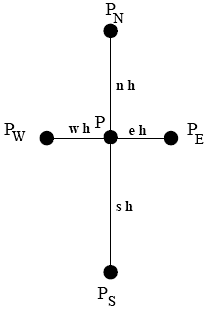
\includegraphics[width=5cm]{Content/Numerik/irregulaereGitter.png}

\end{minipage}
\begin{minipage}{14cm}

$\left(\frac{u(x+eh,y)-u(x,y)}{e(e+w)} +\frac{u(x+wh,y)-u(x,y)}{w(e+w)}+\frac{u(x+nh,y)-u(x,y)}{n(n+s)} + \frac{u(x+sh,y)-u(x,y)}{n(n+s)}\right)\frac{2}{h^2}=f(x,y)$\\

oder
\\

$\frac{u(P_E) - u(P)}{e(e+w)} + \frac{u(P_W) - u(P)}{w(e+w)} + \frac{u(P_N) - u(P)}{n(n+s)} + \frac{u(P_S) - u(P)}{s(n+s)} = \frac{h^2}{2} f(x,y)$
\end{minipage}
\subsubsection{Neumann Rand 
%$\partial_n u(x,y) \forall (x,y) \epsilon \partial_n G$
}
\begin{minipage}{8cm}
	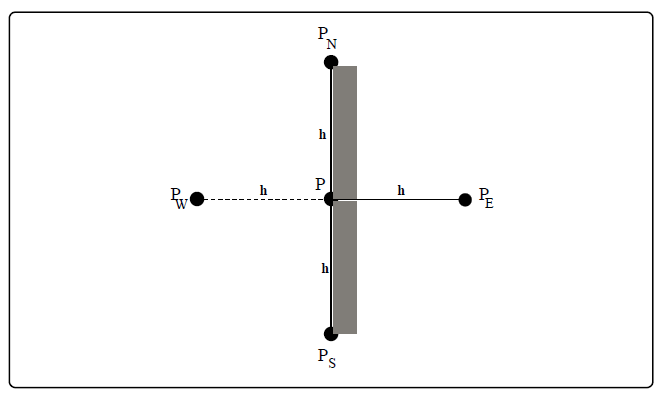
\includegraphics[width=8cm]{Content/Numerik/NeumannRand.png}


\end{minipage}
\begin{minipage}{10cm}
In einem Randpunkt P liegen wie in der Abbildung ersichtlich, $P_N$ und $P_S$ auf dem Rand von Omega, $P_W$ liegt ausserhalb von Omega.\\
In P sei die Neumannsche Randbedingung: $\boxed{\partFrac{u}{n}(P)=g(P)}$\\
$u_x(P)=\frac{u(P_E)-u(P_W)}{2h}\quad\Rightarrow\quad u(P_W)=u(P_E)-2h\cdot u_x(P)$\\

$\boxed{\frac{2u(P_E) + u(P_N) +
u(P_S)- 4 u(P) - 2h\cdot u_x(P)}{h^2}}$\\


\textbf{Spiegelmethode}:\\
Wenn $u_x(x,y) = 0$, dann spricht man auch von der Spiegelmethode. Die Punkte $P_W$ und $P_E$ weisen dann die gleiche Wertigkeit auf ($P_W=P_E$).
\end{minipage}


\subsection{FDM f�r parabolische PDGL}
	W�rmeleitungsgleichung: $\boxed{u_t(x,t)=u_{xx}(x,t)}$\qquad $f(0)=f(1)=0$ \qquad$ \overset{\_}{\Omega}=[0,1]\times [0,\infty]$\\
	
	Randbedingungen: $u(x,0)=f(x) \qquad u(0,t)=u(1,t)=0\qquad x\in(0,1) \qquad t\in[0,\infty)$
\subsubsection{Explizites Verfahren (Richardson-Verfahren)}
$\boxed{\frac{\tilde{u}(x,t+\Delta t) - \tilde{u}(x,t)}{\Delta t} = 
\frac{\tilde{u}(x+\Delta x, t)-2\tilde{u}(x,y) + \tilde{u}( x - \Delta x, t )} {\Delta x^2}} \qquad \Delta x=\frac 1n\qquad \Delta t=\frac r{n^2} \qquad \boxed{r=\frac{\Delta
t}{\Delta x^2}}$\\

\textbf{Idee:} Aus den Positionen k wird k+1 berechnet: $\tilde{u}_{j,k+1} = r \tilde{u}_{j-1,k} + (1-2r)\tilde{u}_{j,k} + r \tilde{u}_{j+1,k}$\\


\begin{itemize}
\item Initialisierung, Randbedingung: $\tilde{u}_{j,0}=f(j/n)$ \qquad $\tilde{u}_{0,k}=\tilde{u}_{n,k}=0$
\item Approximationsmatrize: $C^{(n)}=tridiag_{n-1}(r,1-2r,r)=\begin{bmatrix}
1-2r& r		& 0		& 0 	&\cdots\\
r	& 1-2r  & r		& 0		&\cdots\\
0	& r		& 1-2r 	& r 	&\cdots\\
0	& 0		& r		& 1-2r 	&\cdots\\
\vdots&	\vdots&\vdots&\vdots&\ddots	
\end{bmatrix}$ 
\item Einen Schritt berechnen: $\tilde{u}^{(k+1)}=C^{(n)} \tilde{u}^{(k)}$
\item k-Schritte berechnen: $\tilde{u}^{(k)}=\big\{C^{(n)}\big\}^k \tilde{u}^{(0)}$
\end{itemize}

\textbf{Konvergenzverhalten:} \\

\begin{minipage}{6cm}
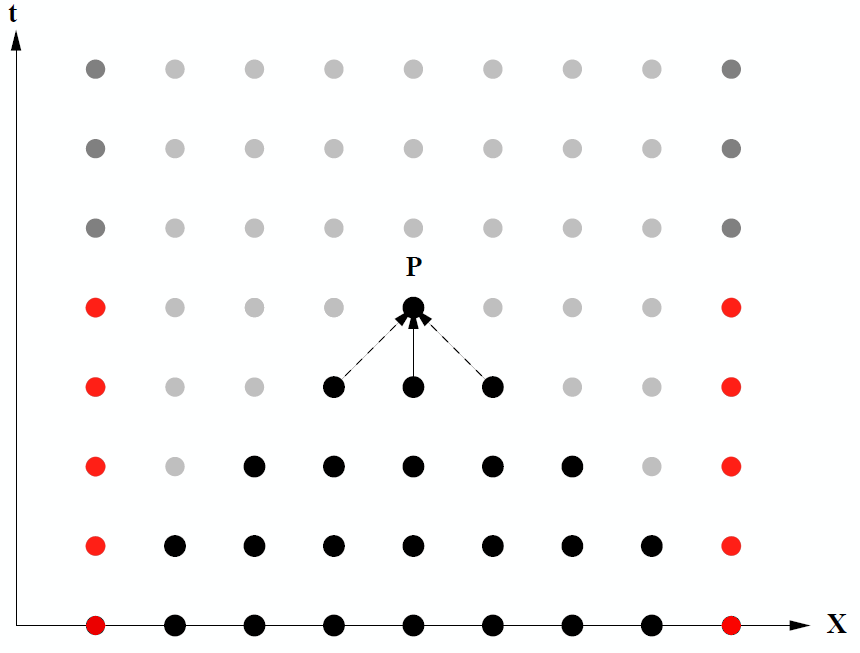
\includegraphics[width=6cm]{Content/Numerik/KonvExplizit.png}
\end{minipage}
\hfill
\begin{minipage}{12cm}
Verfahren ist stabil wenn: $||A^{-1}|| < 1 \qquad \Rightarrow\qquad r < \frac{1}{2}$\\

Dies macht es N�tig die Zeitschritte extrem klein zu w�hlen, darum ist das Verfahren auch nicht wirklich praxistauglich, weil sehr hohe Rechenkapazit�t n�tig sind.\\

Der Grund f�r das schlechte Konvergenzverhalten kann geometrisch visualisiert werden. In die Berechnung des Wertes im Knoten $P$, werden die Werte aller schwarz eingef�rbter Knoten eingehen. Von den Randwerten wird nur die 0-te Stufe ber�cksichtigt.
\end{minipage}






\subsubsection{Implizites Verfahren}
Im Unterschied zum expliziten Verfahren, das Werte vom vorherigen Zeitpunkt nutzt, wird hier das ein Gleichungssystem global gel�st.\\

$\boxed{\frac{\tilde{u}(x,t) - \tilde{u}(x,t -\Delta t)}{\Delta t} = 
\frac{\tilde{u}(x+\Delta x, t)-2\tilde{u}(x,y) + \tilde{u}( x - \Delta x, t )} {\Delta x^2}}$\\

$ \tilde{u}_{j,k} = r \tilde{u}_{j-1,k+1} + (1+2r)\tilde{u}_{j,k+1} + r \tilde{u}_{j+1,k+1}$

\textbf{Idee:} Die Ableitungen werden mittels R�ckw�rtsdifferenz berechnet\\


\begin{itemize}
\item Initialisierung, Randbedingung: $\tilde{u}_{j,0}=f(j/n)$ \qquad $\tilde{u}_{0,k}=\tilde{u}_{n,k}=0$
\item Approximationsmatrize: $E^{(n)}=tridiag_{n-1}(-r,1+2r,-r)=\begin{bmatrix}
1+2r& r		& 0		& 0 	&\cdots\\
r	& 1+2r  & r		& 0		&\cdots\\
0	& r		& 1+2r 	& r 	&\cdots\\
0	& 0		& r		& 1+2r 	&\cdots\\
\vdots&	\vdots&\vdots&\vdots&\ddots	
\end{bmatrix}$ 
\item Einen Schritt berechnen: $\tilde{u}^{(k+1)}=\left\{E^{(n)}\right\}^{-1} \tilde{u}^{(k)}$
\item k-Schritte berechnen: $\tilde{u}^{(k)}=\left(\left\{E^{(n)}\right\}^{-1}\right)^k \tilde{u}^{(0)}$
\end{itemize}

\textbf{Vorteil:} Das implizite Verfahren ist immer stabil, unabh�ngig von der Zeitaufl�sung $\Delta t$\todo{Wirklich immer???}.\\
\textbf{Nachteil:} Aufwendige Matrixinversion n�tig.

\subsubsection{Crank Nicolson -Verfahren (gemischtes Verfahren)}

Die Idee des Verfahrens von Crank-Nicolson ist es die Approximationen\\

$\boxed{\frac{\tilde{u}(x,t+\Delta t) - \tilde{u}(x,t)}{\Delta t} = 
\frac{\tilde{u}(x+\Delta x, t)-2\tilde{u}(x,y) + \tilde{u}( x - \Delta x, t )} {\Delta x^2}}$\\

und\\

$\boxed{\frac{\tilde{u}(x,t) - \tilde{u}(x,t -\Delta t)}{\Delta t} = 
\frac{\tilde{u}(x+\Delta x, t)-2\tilde{u}(x,y) + \tilde{u}( x - \Delta x, t )} {\Delta x^2}}$\\

zu mitteln. Mit dieser Idee geht das stetige Problem in folgendes diskretes Problem �ber:

$-r \tilde{u}_{j-1,k+1} + (2+2r)\tilde{u}_{j,k+1} - r \tilde{u}_{j+1,k+1} = r
\tilde{u}_{j-1,k+1} + (2-2r)\tilde{u}_{j,k+1} + r \tilde{u}_{j+1,k+1} $



\begin{itemize}
\item Initialisierung, Randbedingung: $\tilde{u}_{j,0}=f(j/n)$ \qquad $\tilde{u}_{0,k}=\tilde{u}_{n,k}=0$
\item Approximationsmatrizen:\\
$F^{(n)}=E^{(n)}+I=tridiag_{n-1}(-r,2+2r,-r)=\begin{bmatrix}
2+2r& -r	& 0		& 0 	&\cdots\\
-r	& 2+2r  & -r	& 0		&\cdots\\
0	& -r	& 2+2r 	& -r 	&\cdots\\
0	& 0		& -r	& 2+2r 	&\cdots\\
\vdots&	\vdots&\vdots&\vdots&\ddots	
\end{bmatrix}$\\
$G^{(n)}=C^{(n)}+I=tridiag_{n-1}(~r,~2-2r,~r~)=\begin{bmatrix}
2-2r& r		& 0		& 0 	&\cdots\\
r	& 2-2r  & r		& 0		&\cdots\\
0	& r		& 2-2r 	& r 	&\cdots\\
0	& 0		& r		& 2-2r 	&\cdots\\
\vdots&	\vdots&\vdots&\vdots&\ddots	
\end{bmatrix}$ 
\item Einen Schritt berechnen: $\tilde{u}^{(k+1)}=\left\{F^{(n)}\right\}^{-1} \cdot G^{(n)}\cdot \tilde{u}^{(k)}$
\item k-Schritte berechnen: $\tilde{u}^{(k)}=\left(\left\{F^{(n)}\right\}^{-1} \cdot G^{(n)}\right)^{k}\cdot \tilde{u}^{(0)}$
\end{itemize}

\subsection{(FDM f�r Hyperbolische PDGL)}

$$u_{tt}=u_{xx} = homogen$$
$$u_{tt} -u_{xx}= v(x,t) = inhomogen$$

$$\Longrightarrow u_{j,k+1}=r^2 u_{j-1,k} 2(1-r^2)u_{j,k}+ r^2
u_{j+1,k}-u_{j,k-1}$$
\subsubsection{Anfangsbedingungen}
$$\tilde{u}_{j,0} = f(j\Delta x); u_{j,1}= f(j\Delta x) + g(j\Delta x)\Delta t$$
(f(x)= Anfangsfunktion; g(x)=Ableitung; $r = \frac{\Delta t}{\Delta x}$)

\subsubsection{Transportgleichung}
$$u_x(x,t) + u_t(x, t) = 0; u(x,0)=P(x-t)$$
$$\frac{u(x,t+\Delta t)-u(x,t)}{\Delta t} = \frac{u(x,t) - u(x-\Delta x,
t)}{\Delta x}$$

\clearpage
\section{FEM}

Der Vektorraum $\mathbb{V}$ hat undendlich viele Dimensionen. Falls wir n unabhängige Funktionen $v_1,\ldots,v_n$ wählen, dann spannen die Funktionen $a_1\cdot v_1(x)+\ldots+a_n\cdot v_n(x)$ einen n dimensionalen Teilraum $\mathbb{V}^{(n)}$  von $\mathbb{V}$ auf. Dabei gilt:\\

$\boxed{\tilde{u}^{(n)}=a_1\cdot v_1(x)+\ldots+a_n\cdot v_n(x)}$
\subsection{Das Verfahren von Ritz}
\textbf{Ritzsche Matrize: }
$R^{(n)}=\begin{bmatrix}
	R_{1,1}& R_{1,2}&\cdots\\
	R_{2,1}& R_{2,2}&\cdots\\
	\vdots & \vdots &\ddots\\
\end{bmatrix}$ \qquad mit \qquad $R_{j,k}^{(n)}=\int\limits_{0}^{1}{v_j'(x)\cdot
v_k'(x) dx}$\\
\textbf{Ritzscher Vektor: } 
$r^{(n)}=\begin{bmatrix}
	r_1\\
	r_2\\
	\vdots\\
\end{bmatrix}$ \qquad mit \qquad $r_{k}^{(n)}=\int\limits_{0}^{1}{f(x)\cdot v_k(x) dx}$\\

\textbf{Lösung nach Ritz:} $R^{(n)}\cdot a=r^{(n)}\qquad \Rightarrow \qquad a=\left\{R^{(n)}\right\}^{-1}\cdot r^{(n)}$
\subsection{Das Verfahren von Galerkin}
\textbf{Galerksche Matrize: }
$G^{(n)}=\begin{bmatrix}
	G_{1,1}& G_{1,2}&\cdots\\
	G_{2,1}& G_{2,2}&\cdots\\
	\vdots & \vdots &\ddots\\
\end{bmatrix}$ \qquad mit \qquad $G_{j,k}^{(n)}=\int\limits_{0}^{1}{\underbrace{(v_j''(x))}_{v_j \text{ in Form von DGL!}}\cdot v_k(x) dx}$\\
\textbf{Galerkscher Vektor: } 
$g^{(n)}=\begin{bmatrix}
	g_1\\
	g_2\\
	\vdots\\
\end{bmatrix}$ \qquad mit \qquad $g_{k}^{(n)}=\int\limits_{0}^{1}{f(x)\cdot v_k(x) dx}$\\

\textbf{Lösung nach Galerkin:} $G^{(n)}\cdot a+g^{(n)}=0\qquad \Rightarrow
\qquad a=\textcolor{red}{\mathbf{-}}\left\{G^{(n)}\right\}^{-1}\cdot g^{(n)}$ \quad nach Ritz $G^{(n)} = -R^{(n)} \quad g^{(n)} = r^{(n)}$\\

Die obige Matrix ist nur für die PDGL $-u''(x) = f(x)$ mit dem Ansatz
$\tilde{u}(x) = a_1 \cdot v_1(x) + a_2 \cdot v_2(x)$ gültig. Ansonsten muss ein
Gleichungssystem für $v_k$ = $v_1$ und $v_2$ aufgestellt werden (Beispiel
für DGL: $u''(x) + u(x) + x = 0$):\\
$\int\limits_{0}^{1}{(a_1 \cdot v_1''(x) + a_2 \cdot v_2''(x) + a_1 \cdot
v_1(x) + a_2 \cdot v_2(x) + x) \cdot v_k(x) dx} = 0 \rightarrow G_{j,k}^{(n)}=\int\limits_{0}^{1}(v_j''(x) + v_j(x))\cdot v_k(x) dx$

\subsection{Gewichtete Residuen}
Gewichtungsfunktionen: $\{w_1(x),\ldots,w_n(x)\}$

\textbf{Matrize (gewichtete Residuen): }
$M^{(n)}=\begin{bmatrix}
	M_{1,1}& M_{1,2}&\cdots\\
	M_{2,1}& M_{2,2}&\cdots\\
	\vdots & \vdots &\ddots\\
\end{bmatrix}$ \qquad mit \qquad $M_{j,k}^{(n)}=\int\limits_{0}^{1}{v_j''(x)\cdot w_k(x) dx}$\\
\textbf{Vektor (gewichtete Residuen): } 
$m^{(n)}=\begin{bmatrix}
	m_1\\
	m_2\\
	\vdots\\
\end{bmatrix}$ \qquad mit \qquad $m_{k}^{(n)}=\int\limits_{0}^{1}{f(x)\cdot w_k(x) dx}$\\

\textbf{Lösung der gewichteten Residuen:} $M^{(n)}\cdot a+m^{(n)}=0\qquad \Rightarrow \qquad a=\textcolor{red}{\mathbf{-}}\left\{M^{(n)}\right\}^{-1}\cdot m^{(n)}$

\subsection{Punktkollokation}
Im Sinne einer Punktkollokation (einzelne Punkte müssen zwischen wahrem Resultat und Approximation übereinstimmen) werden $n$ Stützstellen im Intervall von $[0,1]$ gewählt.\\

$\begin{bmatrix}
	v_1''(x_1)& v_2''(x_1)&\cdots\\
	v_1''(x_2)& v_2''(x_2)&\cdots\\
	\vdots& \vdots&\ddots
\end{bmatrix}\cdot
\begin{bmatrix}
a_1\\
a_2\\
\vdots
\end{bmatrix}
=\begin{bmatrix}
-f(x_1)\\
-f(x_2)\\
\vdots
\end{bmatrix}$\qquad Das Gleichungssystem nach a auflösen\\

Die obige Matrix ist nur für die PDGL $-u''(x) = f(x)$ mit dem Ansatz
$\tilde{u}(x) = a_1 \cdot v_1(x) + a_2 \cdot v_2(x)$ gültig. Ansonsten muss die
DGL mit den Ansatzfunktionen aufgestellt und an beiden Punkten eingesetzt
werden, um $a_1$ und $a_2$ zu bestimmen:\\
DGL: $u''(x) + u(x) = -x$ $\Rightarrow$ Gleichung an Punkt 1: $a_1 \cdot
v_1''(x_1) + a_2 \cdot v_2''(x_1) + a_1 \cdot v(x_1) + a_2 \cdot v(x_1) = - x_1$




\subsection{Bereichskollokation}
Im Gegensatz zur Punktkollokation müssen nicht einzelne Punkte sondern ganze Bereiche (Intervalle $I_k$) übereinstimmen. Für $-u''(x) = f(x)$ wird dieses Gleichungssystem aufgestellt.

$\begin{bmatrix}
	\int_{I_1} v_1'' & \int_{I_1} v_2''& \cdots\\
	\int_{I_2} v_1'' & \int_{I_2} v_2''& \cdots\\
	\vdots& \vdots&\ddots
\end{bmatrix}\cdot
\begin{bmatrix}
a_1\\
a_2\\
\vdots
\end{bmatrix}
=\begin{bmatrix}
-\int_{I_1} f(x)\\
-\int_{I_2} f(x)\\
\vdots
\end{bmatrix}$\qquad Das Gleichungssystem nach a auflösen


\subsection{Das Verfahren von Gauss (MSE)}

\textbf{Gausscher Matrize: }
$Q^{(n)}=\begin{bmatrix}
	Q_{1,1}& Q_{1,2}&\cdots\\
	Q_{2,1}& Q_{2,2}&\cdots\\
	\vdots & \vdots &\ddots\\
\end{bmatrix}$ \qquad mit \qquad $Q_{j,k}^{(n)}=\int\limits_{0}^{1}{v_j''(x)\cdot v_k''(x) dx}$\\
\textbf{Gausscher Vektor: } 
$q^{(n)}=\begin{bmatrix}
	q_1\\
	q_2\\
	\vdots\\
\end{bmatrix}$ \qquad mit \qquad $q_{k}^{(n)}=\int\limits_{0}^{1}{f(x)\cdot v_k''(x) dx}$\\

\textbf{Lösung nach Gauss:} $Q^{(n)}\cdot a+q^{(n)}=0\qquad \Rightarrow \qquad a=\textcolor{red}{\mathbf{-}}\left\{Q^{(n)}\right\}^{-1}\cdot q^{(n)}$

\subsection{Finite Elemente}

Die besprochenen Verfahren setzen die Wahl eines Satzes $v_1(x),\ldots,v_n(x)$ von Grundfunktionen voraus. Bei FEM wird mit lokalen Trägern (Grundfunktionen) gearbeitet, diese sind nur auf einem kleinen Intervall ungleich null. Der Vorteil dieses Vorgehens liegt darin, dass in einem Bereich nur ein Träger die Approximationsfunktion beeinflusst. Der Nachteil liegt in der hohen Anzahl der so benötigten Träger.\\

\textbf{WICHTIG:} Alle Verfahren werden mit einer Diskretisierung von $h=1/3$
vorgestellt.

\subsubsection{Knotenvariablen}
Als erstes werden auf dem Intervall $[0,1]$ $n$, normalerweise gleichverteilte, Knotenstellen eingeführt.

\begin{minipage}{11cm}
Dadurch wird das Intervall $[0,1]$ in Teilintervalle (Maschen) zerlegt.\\
 
Für $n=3$:\quad $I_1=[0,1/3]$\quad $I_1=[1/3,2/3]$\quad $I_1=[2/3,1]$\\

Als nächstes wird jeder Knotenstelle $x_k$ eine Ansatzvariable (Knotenvariable) zugeordnet.\\

Ansatz: \quad $\tilde{u}(0)=a_0$\quad $\tilde{u}(1/3)=a_1$\quad $\tilde{u}(2/3)=a_2$\quad $\tilde{u}(1)=a_3$\\

Zusatzbedingungen:
\begin{tabular}{llll}
$v_0(0)=1$&$v_0(1/3)=0$&$v_0(2/3)=0$&$v_0(1)=0$\\
$v_1(0)=0$&$v_1(1/3)=1$&$v_1(2/3)=0$&$v_1(1)=0$\\
$v_2(0)=0$&$v_2(1/3)=0$&$v_2(2/3)=1$&$v_2(1)=0$\\
$v_3(0)=0$&$v_3(1/3)=0$&$v_3(2/3)=0$&$v_3(1)=1$\\
\end{tabular}
\end{minipage}
\hfill
\begin{minipage}{8cm}
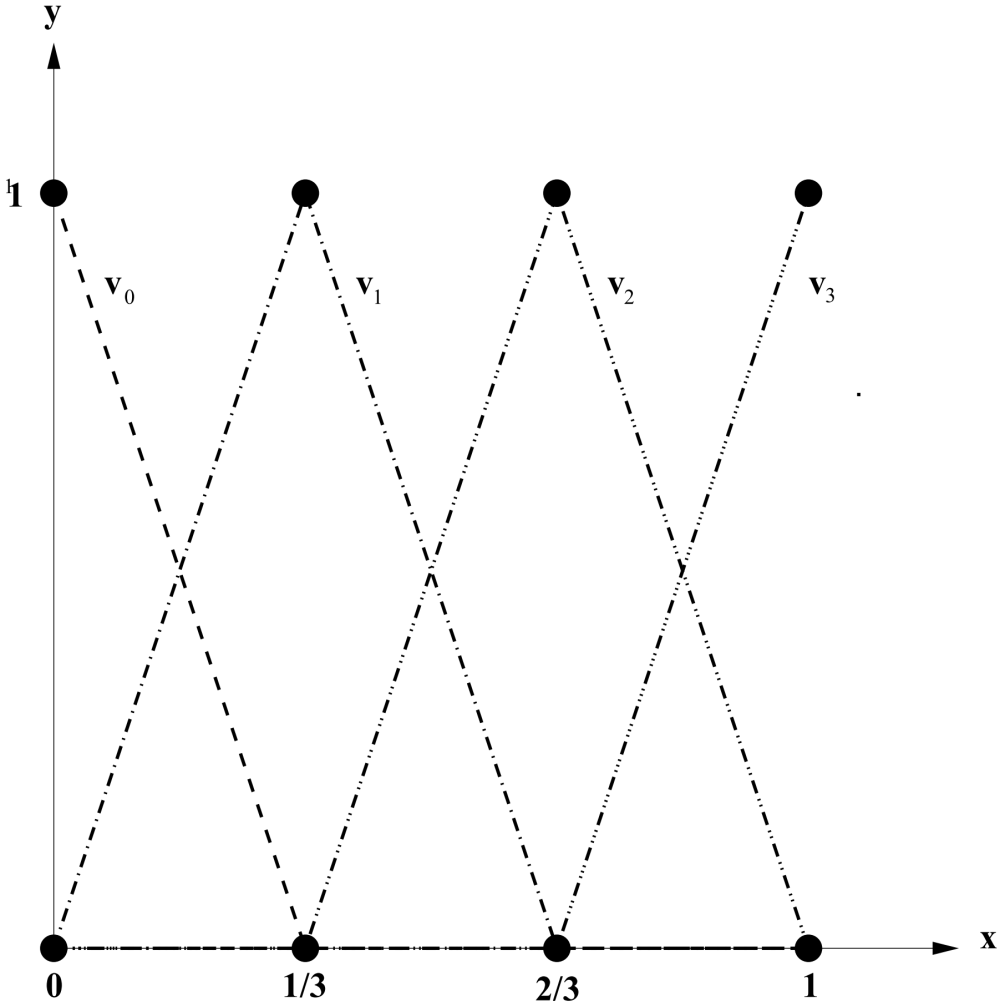
\includegraphics[width=8cm]{Content/Numerik/Traeger1.png}
\end{minipage}


\subsubsection{Formfunktionen}
Die lokalen Grundfunktionen sollen aus Teilstücken einfacher Funktionen, z.B: Polynomen, die nur auf einer einzelnen Masche definiert sind zusammengesetzt werden.\\
Zwei mögliche Formfunktionen sind Beispielsweise:\quad $l_1(x)=1-x$\quad und \quad $l_2(x)=x$\\

\begin{minipage}{8cm}
	\begin{tabular}{lc|c|c}
	$t\in$&$[0,1/3]$&$[1/3,2/3]$&$[2/3,1]$\\
	\hline
	$v_0=$&$1-3x$&$0$&$0$\\
	$v_1=$&$3x$&$2-3x$&$0$\\
	$v_2=$&$0$&$-1+3x$&$3-3x$\\
	$v_3=$&$0$&$0$&$-2+3x$\\
	\end{tabular}
\end{minipage}
\hfill
\begin{minipage}{2cm}
$\Longrightarrow$
\end{minipage}
\hfill
\begin{minipage}{8cm}
	\begin{tabular}{lc|c|c}
	$t\in$&$[0,1/3]$&$[1/3,2/3]$&$[2/3,1]$\\
	\hline
	$v_0=$&$l_1(3x)$&$0$&$0$\\
	$v_1=$&$l_2(3x)$&$l_1(3x-1)$&$0$\\
	$v_2=$&$0$&$l_2(3x-1)$&$l_1(3x-2)$\\
	$v_3=$&$0$&$0$&$l_2(3x-2)$\\
	\end{tabular}
\end{minipage}
\subsubsection{Elementmatrizen}
Grundsätzlich kann die Ansatzvariable durch jedes Verfahren bestimmt werden.
Weil bei einer linearen Ansatzfunktion die zweite Ableitung trivial $(=0)$ ist die Wahl des Ritzschen Verfahren erzwungen.

Die Integrale werden maschenweise ausgewertet:\\

 $\int\limits_{0}^{1}{}=\int\limits_{0}^{1/3}{}+\int\limits_{1/3}^{2/3}{}+\int\limits_{2/3}^{1}{}$\\
 
Durch diesen Ansatz wird die Ritzsche Matrize über jede Masche einzeln berechnet und danach zur globalen Ritzschen Matrize aufsummier:\\

\qquad $R^{(4)}=R^{(4,1)}+R^{(4,2)}+R^{(4,3)}=
\begin{bmatrix}
	* & * & 0 & 0\\
	* & * & 0 & 0\\
	0 & 0 & 0 & 0\\
	0 & 0 & 0 & 0\\
\end{bmatrix}+
\begin{bmatrix}
	0 & 0 & 0 & 0\\
	0 & * & * & 0\\
	0 & * & * & 0\\
	0 & 0 & 0 & 0\\
\end{bmatrix}+
\begin{bmatrix}
	0 & 0 & 0 & 0\\
	0 & 0 & 0 & 0\\
	0 & 0 & * & *\\
	0 & 0 & * & *\\
\end{bmatrix}
$\\

Die mit $*$ bezeichneten $2\times 2$ Matrizen heissen Maschenmatrizen:\\

$M^{(4,1)}=M^{(4,2)}=M^{(4,3)}=
\begin{bmatrix}
	* & *\\
	* & *\\
\end{bmatrix}=3\cdot\begin{bmatrix}
	-1 & 1\\
	1 & -1\\
\end{bmatrix}\qquad\Rightarrow\qquad\boxed{M=\frac 1h\cdot
\underset{\text{\textbf{E}: Elementmatrize}}{\underbrace{\begin{bmatrix}
	-1 & 1\\
	1 & -1\\
\end{bmatrix}}}=\frac 1h\cdot \mathbf{E}}$\\

Die Elementmatrize wird nun in die entsprechende Ritzsche Matrize eingesetzt und überlagert. Für die Quantisierung von $h=1/3$ ergibt sich:\\

$R^{4}=
\begin{bmatrix}
	-3 & 3 & 0 & 0 \\
	3 & -3-3 & 3 & 0 \\
	0 & 3 & -3-3 & 3 \\
	0 & 0 & 3 & -3 \\
\end{bmatrix}=
\begin{bmatrix}
	-3 & 3 & 0 & 0 \\
	3 & -6 & 3 & 0 \\
	0 & 3 & -6 & 3 \\
	0 & 0 & 3 & -3 \\
\end{bmatrix}$\\

Der Ritzsche Vektor muss mittels Integration berechnet werden:\\

$r^4=
\begin{bmatrix}
	\int\limits_{0}^{1}{f(x)\cdot v_0(x)dx}\\
	\int\limits_{0}^{1}{f(x)\cdot v_1(x)dx}\\
	\int\limits_{0}^{1}{f(x)\cdot v_2(x)dx}\\
	\int\limits_{0}^{1}{f(x)\cdot v_3(x)dx}\\
\end{bmatrix}$\\

Das Ritzsche Gleichungssystem dazu ist: $\boxed{R^4\cdot a+r^4=0} \qquad\Rightarrow\qquad a=-\left\{R^4\right\}^{-1}\cdot r^4$\\

\textbf{Anfangsbedingungen:} Die Anfangsbedingungen $a_0$ und $a_n$ können direkt eingesetzt werden.\\

$a_0=10$\qquad$a_3=20$\\

$
	\begin{bmatrix}
		3 & -6 & 3 & 0 \\
		0 & 3 & -6 & 3 \\
	\end{bmatrix}\cdot
	\begin{bmatrix}
		10\\a_1\\a_2\\20
	\end{bmatrix}+r^4=0\qquad\Rightarrow\qquad
	\begin{bmatrix}
		-6 & 3 \\
		 3 & -6 \\
	\end{bmatrix}\cdot
	\begin{bmatrix}
		a_1\\a_2
	\end{bmatrix}+
	\begin{bmatrix}
		30\\60
	\end{bmatrix}+
	r^4=0
$\\

$
	\begin{bmatrix}
			a_1\\a_2
	\end{bmatrix}=
	\begin{bmatrix}
		-6 & 3 \\
	 	 3 & -6 \\
	\end{bmatrix}^{-1}\cdot
	\begin{bmatrix}
		-\left(r^4_1+3\cdot a_0\right)\\
		-\left(r^4_2+3\cdot a_3\right)\\
	\end{bmatrix}		
$

\subsubsection{Die Finite Elemente Handrechnung}
\textbf{Problemstellung:} $u''(x)+f(x)=0\qquad f(x)=20\qquad u(0)=10\qquad u(1)=20$\\

Die Approximation soll auf den \textbf{NICHT} gleichverteilten Intervallen: $[0,1/6]$,\quad $[1/6,1/2]$,\quad $[1/2,1]$\\

Die Entsprechenden Elementmatrizen E sind:\\

$
	\frac{1}{1/6}\begin{bmatrix}
		-1 & 1\\
		1 & -1
	\end{bmatrix}=
	\begin{bmatrix}
			-6 & 6\\
			6 & -6
	\end{bmatrix}\qquad
	\frac{1}{1/2-1/6}\begin{bmatrix}
		-1 & 1\\
		1 & -1
	\end{bmatrix}=
	\begin{bmatrix}
		-3 & 3\\
		3 & -3
	\end{bmatrix}\qquad
	\frac{1}{1-1/2}\begin{bmatrix}
		-1 & 1\\
		1 & -1
	\end{bmatrix}=
	\begin{bmatrix}
		-2 & 2\\
		2 & -2
	\end{bmatrix}
$\\
\\

\begin{minipage}{10cm}
Der Ritzsche Vektor und die Ritzsche Matrize sind:\\

$R^n=
\begin{bmatrix}
		-6 & 6 & 0 & 0\\
		6 & -9 & 3 & 0\\
		0 & 3 & -5 & 2\\
		0 & 0 & 2 & -2\\
\end{bmatrix}$

$
r^n=\begin{bmatrix}
		\int\limits_{0}^{1/6}{f(x)\cdot(1-6x)}dx\\
		\int\limits_{0}^{1/6}{f(x)\cdot(6x)}+\int\limits_{1/6}^{3/6}{f(x)\cdot(3/2-3x)}dx\\
		\int\limits_{1/6}^{3/6}{f(x)\cdot(3x-1/2)}+\int\limits_{3/6}^{1}{f(x)\cdot(2-2x)}dx\\
		\int\limits_{1/2}^{1}{f(x)\cdot(2x-1)}dx\\
\end{bmatrix}=
\begin{bmatrix}
	5/3\\
	5\\
	25/3\\
	5
\end{bmatrix}
$\end{minipage}
\hfill
\begin{minipage}{9cm}
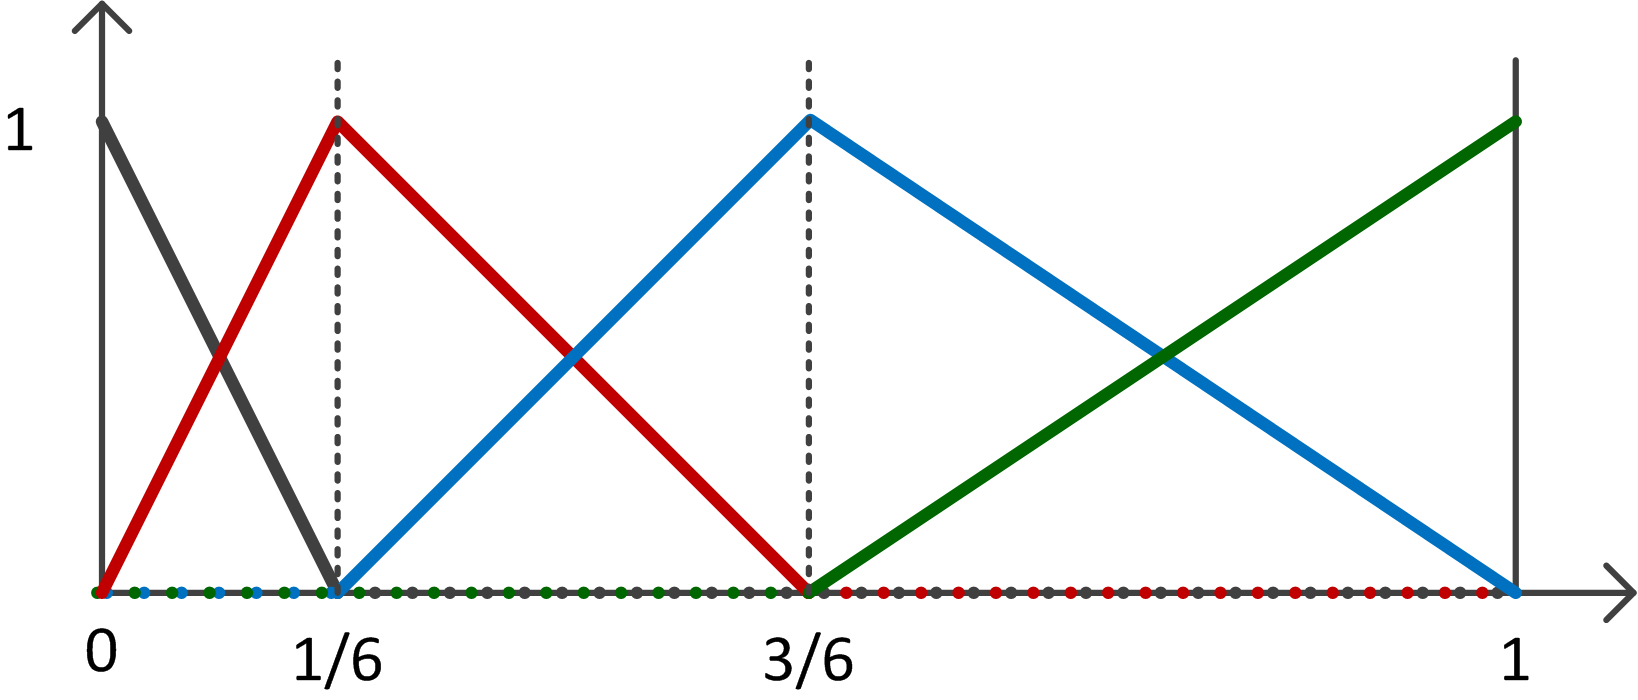
\includegraphics[width=9cm]{Content/Numerik/FEMHand}
\end{minipage}\\

$R^n\cdot a +r^n=0 \qquad\Rightarrow\qquad
\begin{bmatrix}
	-6 & 6 & 0 & 0\\
	6 & -9 & 3 & 0\\
	0 & 3 & -5 & 2\\
	0 & 0 & 2 & -2\\
\end{bmatrix}\cdot
\begin{bmatrix}
	10\\
	a_1\\
	a_2\\
	20
\end{bmatrix}+
\begin{bmatrix}
	5/3\\
	5\\
	25/3\\
	5
\end{bmatrix}=
\begin{bmatrix}
	0\\
	0\\
	0\\
	0
\end{bmatrix}\qquad\Rightarrow\qquad
\begin{bmatrix}
	6 & -9 & 3 & 0\\
	0 & 3 & -5 & 2\\
\end{bmatrix}\cdot
\begin{bmatrix}
	10\\
	a_1\\
	a_2\\
	20
\end{bmatrix}+
\begin{bmatrix}
	5/3\\
	5\\
	25/3\\
	5
\end{bmatrix}=
\begin{bmatrix}
	0\\
	0\\
	0\\
	0
\end{bmatrix}	
$\\
\\

$\qquad\Rightarrow\qquad
\begin{bmatrix}
	-9 & 3\\
	3 & -5\\
\end{bmatrix}\cdot
\begin{bmatrix}
	a_1\\
	a_2\\
\end{bmatrix}+
\begin{bmatrix}
	6\cdot 10\\
	2\cdot 20\\
\end{bmatrix}+
\begin{bmatrix}
	5\\
	25/3\\
\end{bmatrix}
=0\qquad\Rightarrow\qquad
\begin{bmatrix}
	-9 & 3\\
	3 & -5\\
\end{bmatrix}\cdot
\begin{bmatrix}
	a_1\\
	a_2\\
\end{bmatrix}=
\begin{bmatrix}
	-65\\
	-145/3\\
\end{bmatrix}\qquad\Rightarrow\qquad
\begin{bmatrix}
	a_1\\
	a_2\\
\end{bmatrix}=
\begin{bmatrix}
	235/18\\
	35/2\\
\end{bmatrix}
$\\
\\
$
\qquad\Rightarrow\qquad \tilde{u}(x)=10\cdot v_0(x)+\frac{235}{18} v_1(x)+\frac{35}{2}\cdot v_2(x)+20\cdot v_3(x)=
$




\subsubsection{h-Strategie}

Die Grundidee der h-Strategie ist die Verfeinerung der Auflösung. Mit anderen Worten die Maschenbreite $h$ wird verkleinert. Um den ganzen Bereich dennoch abdecken zu können sind mehr Maschen notwendig.

\subsubsection{p-Strategie}
Bei der p-Strategie bleibt das Netz bestehen. Die Ansatzfunktionen sollen nun durch Polynome höherer Ordnung zusammengesetzt werden, dazu werden neue Knoten und Knotenvariablen eingeführt werden.\\

\textbf{Problemstellung:} $u''(x)+f(x)=0\qquad u(0)=a_0\qquad u(1)=a_6$\\

Die Approximation soll auf dem gleichverteilten Intervallen gelten: $[0,1/3]$,\quad $[1/3,2/3]$,\quad $[2/3,1]$\\

\begin{minipage}{4cm}
	Formfunktionen:\\

	$q_1(x)=(1-x)\cdot(1-2x)$\\
	$q_2(x)=4x\cdot(1-x)$\\
	$q_3(x)=-x\cdot(1-2x)$\\
	
	Elementmatrize: $\boxed{E=\frac{1}{3}
	\begin{bmatrix}
		-7& 8 & -1\\
		8& -16& 8\\
		-1& 8& -7	
	\end{bmatrix}}$\\
\end{minipage}
\hfill
\begin{minipage}{8cm}
	\begin{tabular}{lc|c|c}
		$x\in$&$[0,1/3]$&$[1/3,2/3]$&$[2/3,1]$\\
		\hline
		$v_0=$&$q_1(3x)$&$0$&$0$\\
		$v_1=$&$q_2(3x)$&$0$&$0$\\
		$v_2=$&$q_3(3x)$&$q_1(3x-1)$&$0$\\
		$v_3=$&$0$&$q_2(3x-1)$&$0$\\
		$v_4=$&$0$&$q_3(3x-1)$&$q_1(3x-2)$\\
		$v_5=$&$0$&$0$&$q_2(3x-2)$\\
		$v_6=$&$0$&$0$&$q_3(3x-2)$\\
	\end{tabular}
\end{minipage}
\hfill
\begin{minipage}{6cm}
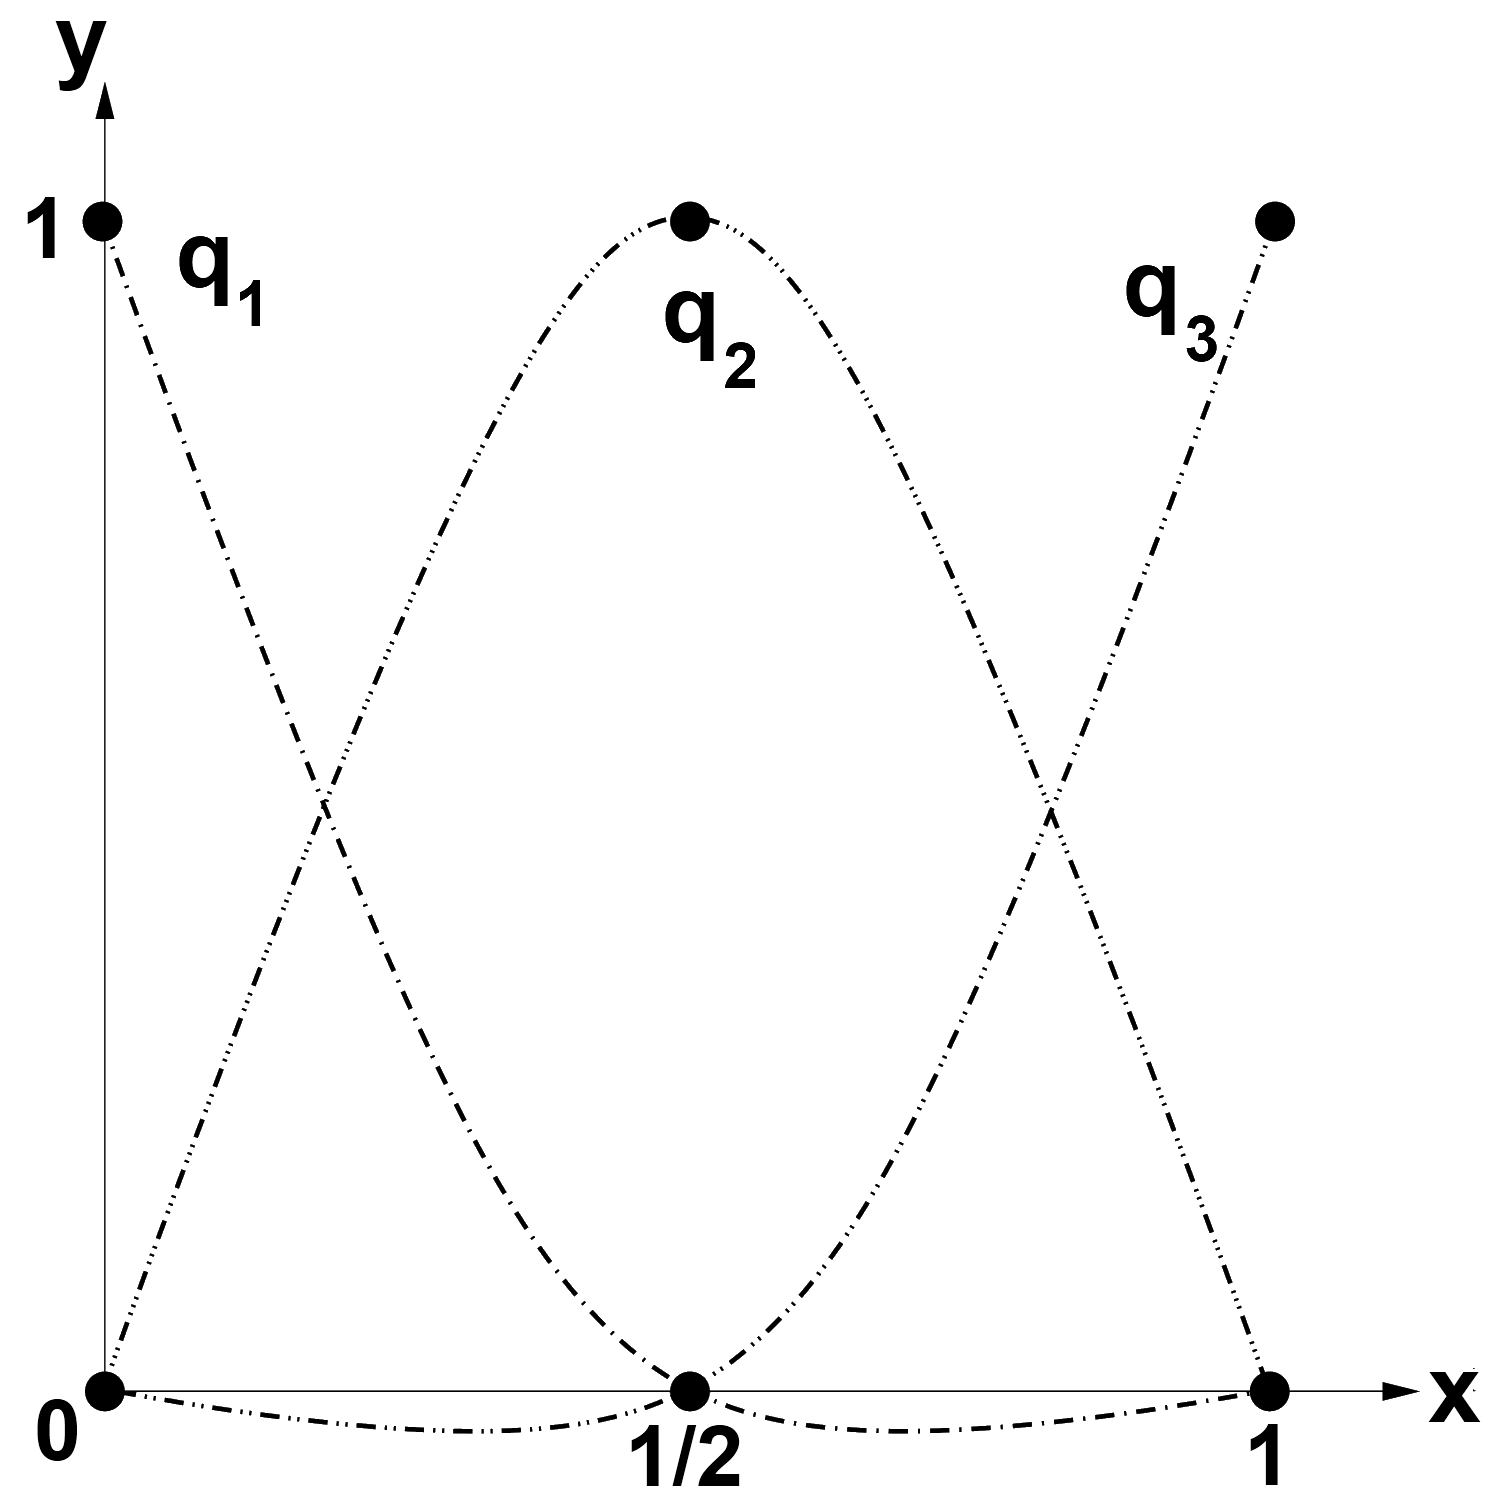
\includegraphics[width=6cm]{Content/Numerik/FEM2Ord}
\end{minipage}\\

$\underset{\text{Ritzsche Matrize $R^{(8)}$ für } h=1/3}{\underbrace{\begin{bmatrix}
	-7& 8 & -1& 0& 0& 0& 0\\
	 8& -16& 8& 0& 0& 0& 0\\
	-1& 8& -14& 8& -1& 0& 0\\ 
	 0& 0& 8& -16& 8& 0& 0\\
	 0& 0& -1& 8& -14& 8& -1\\ 
	 0& 0& 0& 0& 8& -16& 8\\
	 0& 0& 0& 0& -1& 8& -7	
\end{bmatrix}}}\cdot\begin{bmatrix}
	a_0\\
	a_1\\
	a_2\\
	a_3\\
	a_4\\
	a_5\\
	a_6\\
\end{bmatrix}
+\underset{\text{Ritzscher Vektor $r^{(8)}$ für } h=1/3}{\underbrace{\begin{bmatrix}
	\int\limits_{0}^{1}{f(x)\cdot v_0(x)dx}\\
	\int\limits_{0}^{1}{f(x)\cdot v_1(x)dx}\\
	\int\limits_{0}^{1}{f(x)\cdot v_2(x)dx}\\
	\int\limits_{0}^{1}{f(x)\cdot v_3(x)dx}\\
	\int\limits_{0}^{1}{f(x)\cdot v_4(x)dx}\\
	\int\limits_{0}^{1}{f(x)\cdot v_5(x)dx}\\
	\int\limits_{0}^{1}{f(x)\cdot v_6(x)dx}\\
\end{bmatrix}}}=
\begin{bmatrix}
	0\\
	0\\
	0\\
	0\\
	0\\
	0\\
	0\\
	0\\
\end{bmatrix}
$\\

\textbf{Vorteil der p-Strategie gegenüber der h-Strategie:} Bei beiden Strategien steigt die Dimension der Systemmatrizen an. Es besteht jedoch die berechtigte Hoffnung, dass der Zuwachs der benötigt wird, um eine vergleichbare Genauigkeit zu errreichen, bei der p-Strategie weitaus geringer ist als bei der h-Strategie. 

\subsection{Konformität und Vollständigkeit}
Muss nun die Approximationslösung zweimal ableitbar sein, so gilt der Ansatz des letzten Abschnitt nicht mehr als konform.

Um die einmalige Differenzierbarkeit an den Knoten zu gewährleisten müssen neue Grundfunktionen gefunden werden.\\

$\tilde{u}(x)=a_0v_0(x)+a_1v_1(x)+a_2v_2(x)+a_3v_3(x)+\tilde{a}_0\tilde{v}_0(x)+\tilde{a}_1\tilde{v}_1(x)+\tilde{a}_2\tilde{v}_2(x)+\tilde{a}_3\tilde{v}_3(x)$\\

Zwei Grundfunktionen stellen den richtigen Wert and den Knoten sicher. Zwei weitere Grundfunktionen werden benötigt um die erste Ableitung (Steigung) an den Übergangknoten sicherzustellen, sie sorgen für die Vollständigkeit der Grundfunktionen. (Ohne die zwei weiteren Grundfunktionen wäre an den Übergangsknoten nur eine Steigung von Null möglich.)

\subsection{Hermetische Polynome dritter Ordnung}
Übereinstimmung bis zur 1.Ableitung an den Knotenpunkten\\

\textbf{Problemstellung:} $u''(x)+f(x)=0\qquad u(0)=a_0\qquad u'(0)=\tilde{a}_0 \qquad u(1)=a_3\qquad  u'(1)=\tilde{a}_3$\\

Die Approximation soll auf dem gleichverteilten Intervallen gelten: $[0,1/3]$,\quad $[1/3,2/3]$,\quad $[2/3,1]$\\

\begin{minipage}{4cm}
Formfunktionen:\\
$h_1(x)=2x^3-3x^2+1$\\
$h_2(x)=x^3-2x^2+x$\\
$h_3(x)=-2x^3+3x^2$\\
$h_4(x)=x^3-x^2$
\end{minipage}
\hfill
\begin{minipage}{8cm}
	\begin{tabular}{lc|c|c}
		$x\in$&$[0,1/3]$&$[1/3,2/3]$&$[2/3,1]$\\
		\hline
		$v_0=$&$h_1(3x)$&$0$&$0$\\
		$\tilde{v}_0=$&$\frac 13 h_2(3x)$&$0$&$0$\\
		$v_1=$&$h_3(3x)$&$h_1(3x-1)$&$0$\\
		$\tilde{v}_1=$&$\frac 13 h_4(3x)$&$\frac 13 h_2(3x-1)$&$0$\\
		$v_2=$&$0$&$h_3(3x-1)$&$h_1(3x-2)$\\
		$\tilde{v}_2=$&$0$&$\frac 13 h_4(3x-1)$&$\frac 13 h_2(3x-2)$\\
		$v_3=$&$0$&$0$&$h_3(3x-2)$\\
		$\tilde{v}_3=$&$0$&$0$&$\frac 13 h_2(3x-1)$\\
	\end{tabular}
\end{minipage}
\hfill
\begin{minipage}{6cm}
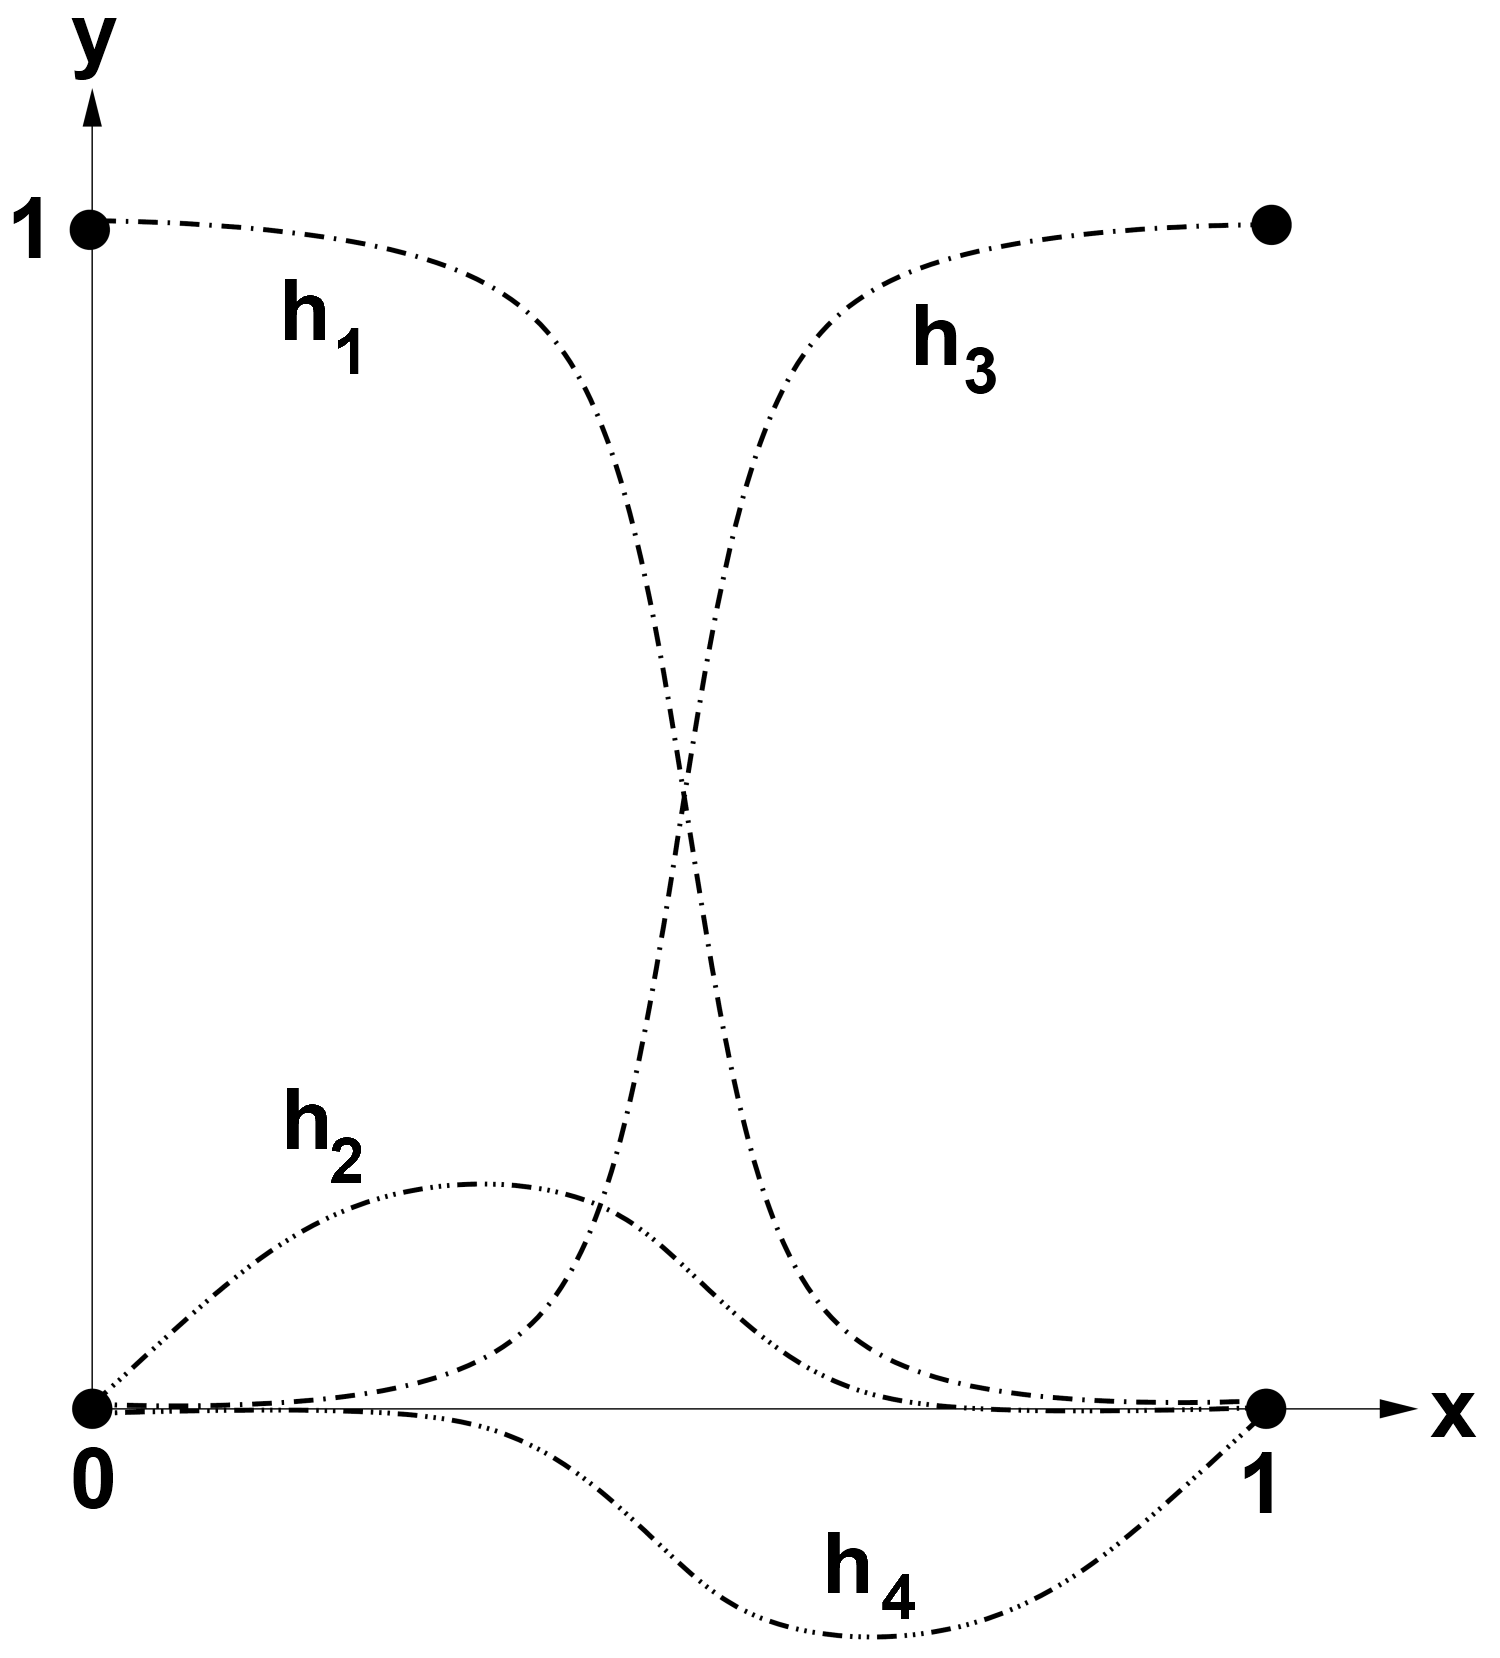
\includegraphics[width=6cm]{Content/Numerik/FEM3Ord}
\end{minipage}\\
$E=\frac{1}{30}
\begin{bmatrix}
	-36 & -3 & 36 & -3\\
	-3 & -4 & 3 & 1\\
	36 & 3 & -36 & 3\\
	-3 & 1 & 3 & -4\\
\end{bmatrix}\qquad\Rightarrow\qquad
\boxed{M=\frac{1}{30\cdot h}
\begin{bmatrix}
	-36 & -3\cdot h & 36 & -3\cdot h\\
	-3\cdot h & -4\cdot h^2 & 3\cdot h & 1\cdot h^2\\
	36 & 3\cdot h & -36 & 3\cdot h\\
	-3\cdot h & 1\cdot h^2 & 3\cdot h & -4\cdot h^2\\
\end{bmatrix}}$\\
\\


$\underset{\text{Ritzsche Matrize $R^{(8)}$ für } h=1/3}{\underbrace{\frac{3}{30}\begin{bmatrix}
	-36 & -1 & 36 & -1 & 0  & 0  & 0  & 0 \\
	-1  & -4/9  & 1  & 1/9  & 0  & 0  & 0  & 0\\
	36  & 1  & -72  & 0  & 36  & -1  & 0  & 0\\
	-1  & 1/9  & 0  & -8/9  & 1  & 1/9  & 0  & 0\\
	0  & 0  & 36  & 1  & -72  & 0  & 36  & -1\\
	0  & 0  & -1  & 1/9  & 0  & -8/9  & 1  & 1/9\\
	0  & 0  & 0  & 0  & 36  & 1  & -36  & 1\\
	0  & 0  & 0  & 0  & -1  & 1/9  & 1  & -4/9\\
\end{bmatrix}}}\cdot\begin{bmatrix}
	a_0\\
	\tilde{a}_0\\
	a_1\\
	\tilde{a}_1\\
	a_2\\
	\tilde{a}_2\\
	a_3\\
	\tilde{a}_3\\
\end{bmatrix}
+\underset{\text{Ritzscher Vektor $r^{(8)}$ für } h=1/3}{\underbrace{\begin{bmatrix}
	\int\limits_{0}^{1}{f(x)\cdot v_0(x)dx}\\
	\int\limits_{0}^{1}{f(x)\cdot \tilde{v}_0(x)dx}\\
	\int\limits_{0}^{1}{f(x)\cdot v_1(x)dx}\\
	\int\limits_{0}^{1}{f(x)\cdot \tilde{v}_1(x)dx}\\
	\int\limits_{0}^{1}{f(x)\cdot v_2(x)dx}\\
	\int\limits_{0}^{1}{f(x)\cdot \tilde{v}_2(x)dx}\\
	\int\limits_{0}^{1}{f(x)\cdot v_3(x)dx}\\
	\int\limits_{0}^{1}{f(x)\cdot \tilde{v}_3(x)dx}\\
\end{bmatrix}}}=
\begin{bmatrix}
	0\\
	0\\
	0\\
	0\\
	0\\
	0\\
	0\\
	0\\
\end{bmatrix}
$\\







%\subsection{FEM für parabolische PDEs}
\newpage
\section{Fourierreihe}
  	Komplex: $$\boxed{f(t) = \sum\limits_{k = -\infty}^{\infty} c_k \cdot e^{j k
  	\omega_f t}}= \sum\limits_{k = 0}^{\infty} \left(c_k \cdot e^{j k \omega_f
  	t} + \overline{c_k} \cdot e^{-j k \omega_f t}\right) \quad
  	\boxed{c_k=\overline{c_{-k}}=\frac{1}{T}\int_0^T{f(t)\cdot
	e^{-jk\omega_f t}dt}}$$
	
	\vspace{0.5cm}
	
  	Reell: $$\boxed{f(t) = \frac{a_0}{2} + \sum\limits_{k=1}^{\infty} \left[a_k
  	\cos(k \omega_f t) + b_k \sin(k \omega_f t)\right]}=\frac{A_0}{2} +
  	\sum\limits_{k=1}^{\infty} A_k \cos(k \omega_f t + \varphi_k) \quad k\in
  	\mathbb{Z}$$	
	
	$$\boxed{a_0 =
	\frac{2}{T}\int\limits_0^{T} f(t)dt, \quad a_k = \frac{2}{T}\int\limits_0^{T} f(t)\cos(k \omega_f t) dt, \quad b_k =
	\frac{2}{T}\int\limits_0^{T} f(t)\sin(k \omega_f t) dt} \quad
	\boxed{\omega_f=\frac{2 \pi}{T}=2 \pi f}$$
	
	\vspace{0.5cm}

	$a_0$, $c_0$, $A_0$ sind \textit{Konstanten}, $\omega_f$ ist die
	\textit{Grundkreisfrequenz}, $a_k$ und $b_k$ sind die \textit{reellen
	Koeffizienten}, $c_k$ ist der \textit{komplexe Koeffizient}, $A_k$ ist die
	\textit{Amplitude} und $\varphi_k$ ist die \textit{Phase}.\\
	\fbox{
	\begin{tabular}{p{9cm}p{9cm}}
		$a_k = c_k + \bar{c_k} = 2\Real(c_k) = A_k \cos(\varphi_k)$ &
		$b_k = j(c_k + \bar{c_k}) = -2\Imag(c_k) = -A_k \sin(\varphi_k)$ \\ \\
		$c_k = \frac{a_k-jb_k}{2} = \frac{A_k}{2} e^{j\varphi_k}$ &
		$c_{-k} = \overline{c_k} = \frac{a_k+jb_k}{2} = \frac{A_k}{2} e^{-j\varphi_k}$ \\ \\
		$A_k = 2|c_k| = \sqrt{a_k^2+b_k^2}$
	\end{tabular}}\\

	\textbf{Berechnung von $\varphi_k$ aus $a_k$ und $b_k$}\\
	\begin{tabular}{|p{4cm}p{4cm}|p{3cm}p{3.5cm}|}
		\hline
		$a_k> 0:$ & $\varphi_k = -\arctan(\frac{b_k}{a_k})$ &
		$a_k<0:$ &	$\varphi_k = -\arctan(\frac{b_k}{a_k}) + \pi$\\
		\hline
		$a_k = 0; b_k > 0:$ &	$\varphi_k = -\frac{\pi}{2}$ &
		$a_k = 0; b_k < 0:$ &	$\varphi_k = \frac{\pi}{2}$\\
		\hline
		$a_k = b_k = 0:$ &	$\varphi_k = \text{nicht definiert}$ & & $\varphi_k =
		arg(c_k)$\\
		\hline
	\end{tabular}

	\subsection{Symmetrie}
		\begin{tabular}{|p{4.3cm}|p{4.3cm}|p{4.4cm}|p{4.4cm}|}
         	\hline
        	\textbf{gerade Funktion} & \textbf{ungerade Funktion} &
        	\textbf{Halbperiode 1} & \textbf{Halbperiode 2}\\
        	\hline
        	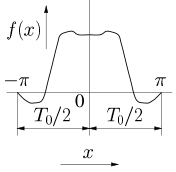
\includegraphics[width=3cm]{Content/Transformationen/gerade_funktion.png}&
        	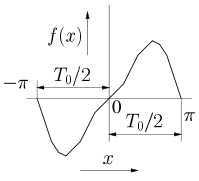
\includegraphics[width=3cm]{Content/Transformationen/ungerade_funktion.png}&   
 			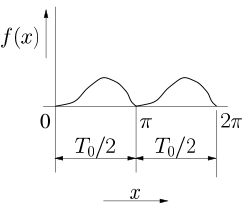
\includegraphics[width=3cm]{Content/Transformationen/halbperiode_1.png}&   
			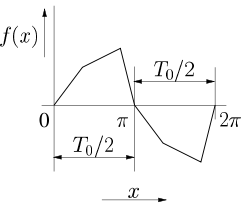
\includegraphics[width=3cm]{Content/Transformationen/halbperiode_2.png}\\
			\hline & & & \\			
   			$f(-t)=f(t)$ & $f(-t)=-f(t)$ & $f(t)=f(t+\pi)$ & $f(t)=-f(t+\pi)$\\
   			$b_k=0$ & $a_k=0$ & $a_{2k+1}=0$ & $a_{2k}=0$\\
   			$a_k = \frac{4}{T} \int\limits_0^{\frac{T}{2}} f(t) \cdot \cos(k \omega_f
   			t) dt$ &
   			$b_k =  \frac{4}{T} \int\limits_0^{\frac{T}{2}} f(t) \cdot
			\sin(k \omega_f t) dt$ &
			$b_{2k+1}=0$ & $b_{2k}=0$\\
			\hline
      	\end{tabular} 
     	
   \subsection{Spektern}
   	\begin{tabular}{p{6cm} p{6cm} p{6cm}}
   		Kosinus- Sinusamplitudenspektrum & 
   		Einseitiges Amplituden-/ Phasenspek. &
   		Zweiseitges Amplituden-/ Phasenspek. \\
   		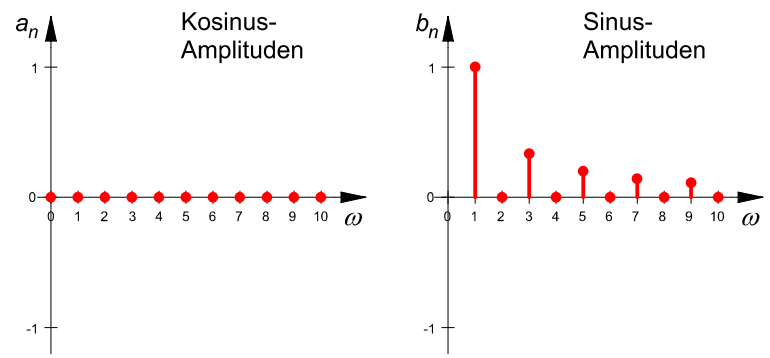
\includegraphics[width=5cm]{Content/Transformationen/cosSinSpectr.png} &
   		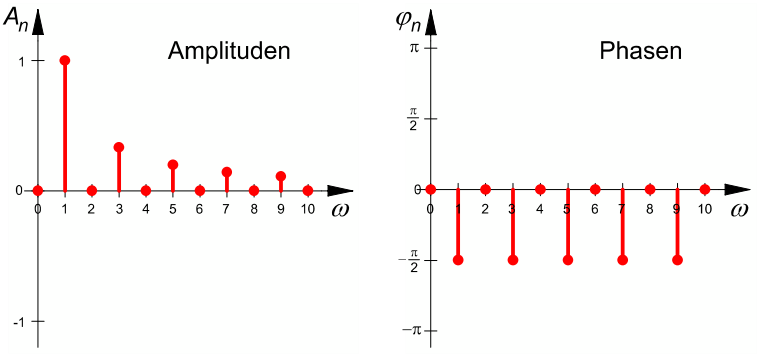
\includegraphics[width=5cm]{Content/Transformationen/EinseitigSpectr.png} &
   		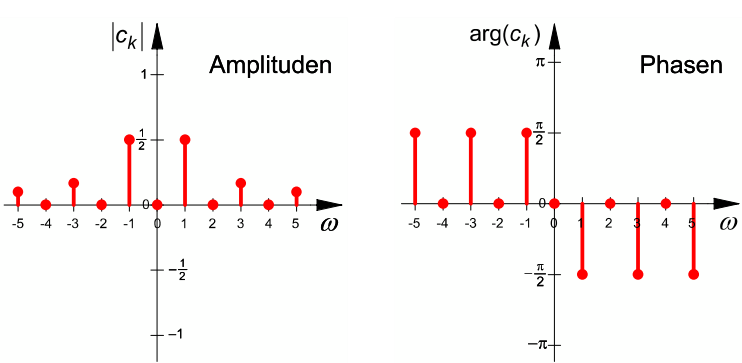
\includegraphics[width=5cm]{Content/Transformationen/ZweiseitigSpectr.png}
   	\end{tabular}
   	Das einseitige und zweiseitige Spektrum unterscheiden sich nur im
  	Amplitudendiagramm. Das Phasendiagramm f"ur positive $k$ ist identisch. Die
  	Amplidudenwerte sind h"alftig auf die pos. und neg. $k$ verteilt.
 
\section{Fourier Transformation}
	$$\boxed{f(t) =  \frac{1}{2\pi}\int\limits_{-\infty}^{\infty}
	F(\omega)e^{j\omega t}d\omega}=\frac{1}{2
	\pi}\int\limits_{-\infty}^{\infty}[R(\omega) \cos(\omega t) + X(\omega)
	\sin(\omega t)]d\omega + \frac{j}{2 \pi}\int \limits_{-
	\infty}^{\infty}[R(\omega) \sin(\omega t)- X(\omega) \cos(\omega t)]d\omega$$
	
	$$\boxed{F(\omega) = \int\limits_{-\infty}^{\infty} f(t)e^{-j\omega t}dt}
	= R(\omega) - j X(\omega) \quad R(\omega) = \int\limits_{-\infty}^{\infty}
	f(t)\cos(\omega t)dt \quad \mbox{ und } \quad X(\omega)=
	\int\limits_{-\infty}^{\infty}f(t)\sin(\omega t)dt$$
	\begin{tabular}{lllll}
	 $ \sigma(t) \FT \frac{1}{j\omega}+\pi \cdot \delta(\omega) $ & \hspace{6mm} &
	 $ \frac{1}{\pi \cdot t} \FT -j \cdot sgn(\omega) $ & \hspace{6mm} &  \\ 
	 $ 1 \FT 2\pi \cdot \delta(t) \underbrace{\longleftrightarrow}_{Vorsichtig}
	 \delta(\omega) \FT 1 $ & & $ sgn(t) \FT \frac{2}{j\omega} $
	\end{tabular}
		
	\subsection{Eigenschaften}
		Fourierintegral existiert wenn  $\int\limits_{-\infty}^{\infty}|f(t)| dt <
	\infty$\\
		\renewcommand{\arraystretch}{2}
		\begin{tabular}{|p{8cm}|l c l|}
        	\hline
        	Linearit"at & 
        	$\alpha\cdot f(t) + \beta\cdot g(t)$ & $\FT$ & $\alpha\cdot F(\omega) +
        	\beta\cdot G(\omega)$\\
        	\hline
			Zeitumkehrung (Spiegelung an der Y-Achse)&
			$f(-t)$ & $\FT$ & $F(-\omega) = F^*(\omega)$ \\
			\hline        	
  			"Ahnlichkeit &
  			$f(\alpha t)$ & $\FT$ & $\frac{1}{|\alpha|}F \left (\frac{\omega}{\alpha} \right)
  			\quad\alpha \in\mathbb{R}\setminus \{0\}$\\
  			\hline
  			Verschiebung im	Zeitbereich &
  			$f(t\pm t_0)$ & $\FT$ & $F(\omega)e^{\pm j\omega t_0}$\\
  			\hline
			Verschiebung im Frequenzbereich &
			$f(t)e^{\pm j\omega_0 t}$ & $\FT$ & $F(\omega\mp\omega_0)$\\
			\hline
			Ableitung im Zeitbereich &
			$\frac{\partial^n f(t)}{\partial t^n}$ & $\FT$ & $(j\omega)^n F(\omega)$\\
			\hline
			Integration im Zeitbereich &
			$\int\limits_{-\infty}^{t}f(\tau)d\tau $ & $\FT$ & 
			$\frac{F(\omega)}{j\omega}+\pi F(0)\delta(\omega)$\\
			\hline				
			Ableitung im Frequenzbereich &
			$t^n f(t)$ & $\FT$ & $j^n \frac{\partial F(\omega)}{\partial \omega^n}$\\
			\hline		
			Faltung im Zeitbereich &
			$f(t) \ast g(t)$ & $\FT$ & $F(\omega) \cdot G(\omega)$\\
			\hline
			Faltung im Frequenzbereich &
			$f(t) \cdot g(t)$ & $\FT$ & $\frac{1}{2\pi}F(\omega) \ast G(j\omega)$\\
			\hline
			Vertauschungssatz (Dualit�t) &
			$f(t)$ & $\FT$ & $F(\omega)\nonumber$ \\
 			& $F(t)$ & $\FT$ & $2\pi \cdot f(-\omega)$\\
 			\hline
 			Modulation &
 			$\cos(\alpha t) \cdot f(t)$ & $\FT$ & $\frac{1}{2}\cdot
 			\left[F(\omega-\alpha) + F(\omega+\alpha)\right ]$\\
 			& $\sin(\alpha t) \cdot f(t)$ & $\FT$ & $\frac{1}{2j}\cdot \left[
 			F(\omega-\alpha) - F(\omega+\alpha)\right ]$\\
 			\hline
        	Parseval's Theorem &
 			$\int\limits_{-\infty}^{\infty}f(t)g^{\ast}(t)dt $ & $=$ & $ \frac{1}{2\pi}
  			\int\limits_{-\infty}^{\infty}F(\omega)G^{\ast}(\omega)d\omega$\\
  			\hline
  			Bessel's Theorem (Satz von Parseval) &
  			$\int\limits_{-\infty}^{\infty}|f(t)|^2 dt $ & $=$ & $ \frac{1}{2\pi}
  			\int\limits_{-\infty}^{\infty}|F(\omega)|^2 d\omega$\\
  			\hline 			
			Anfangswerte &
			$f(0)=\frac{1}{2\pi}\int\limits_{-\infty}^{\infty}F(\omega)d\omega
			$ && $ F(0)=\int\limits_{-\infty}^{\infty}f(t)dt$\\
			\hline
			$\infty$ lange Folge von $\delta$-Impulsen &
			$\sum\limits_{n=-\infty}^{\infty} \delta(t-n\cdot t_0)$ & $\FT$ & 
			$\sum\limits_{n=-\infty}^{\infty}
			\frac{2\pi}{t_0}\delta(\omega-n\cdot \frac{2\pi}{t_0})$\\
			\hline
        \end{tabular}
		\renewcommand{\arraystretch}{1}
		
	
\section{Laplace Transformation}
	$$\boxed{F(s)=\int\limits_0^\infty f(t)e^{-st}dt} \qquad s=\sigma +j\omega$$\\
	- Definitionsbereich nur f"ur \textbf{kausale} Systeme $\boxed{t\geq 0}$\\
	- Integrierbar "uber das Intervall $(0,\infty)$\\
	- Wachstum kleiner als der von eienr Exponentialfunktion $\boxed{\sigma > 0}$\\
	- $\sigma$ ist der D"ampfungsfaktor: $e^{-s}=e^{-\sigma} \cdot e^{-j\omega}$ \\
	- Fourier-Transformierte $F(\omega)$ kann durch die
	Laplace-Transformation $F(s)$ ausgedr"uckt werden.  \\
	- Fourier $\longleftrightarrow$ Laplace Umwandlungen nur wenn Polstelle
	($\sigma > 0$) dh. links von $j\omega$ Achse und kausal!
  
 	\subsection{Eigenschaften}
  		\renewcommand{\arraystretch}{2}
		\begin{tabular}{|l|l c p{5.5cm}|}
        	\hline
        	Linearit"at & 
 			$\alpha\cdot f(t) + \beta\cdot g(t)$ & $\FT$ & $\alpha\cdot F(s) +
 			\beta\cdot G(s)$ \\
 			\hline
 			Verschiebung im Zeitbereich &
 			$f(t\pm t_0) $ & $\FT$ & $ F(s)e^{\pm t_0 s}$ \\
 			\hline
 			D"ampfung (Verschiebung im Frequenzbereich) &
 			$f(t)e^{\mp\alpha t}$ & $\FT$ & $F(s\pm\alpha)$ \\
 			\hline
 			"Ahnlichkeit&
 			$f(\alpha t)$ & $\FT$ & $\frac{1}{\alpha}F \left (\frac{s}{\alpha} \right )
 			\quad 0 <\alpha \in\mathbb{R}$ \\
 			\hline
 			Faltung im Zeitbereich &
 			$f(t) \ast g(t)$ & $\FT$ &
 			$F(s) \cdot G(s)$\\
 			\hline 			
 			Faltung im Frequenzbereich &
 			$f(t) \cdot g(t)$ & $\FT$ & $\frac{1}{2 \pi j} F(s) \ast G(s)$ \\
 			\hline
 			Differentiation im Zeitbereich &
 			$f'(t)$ & $\FT$ & $sF(s) - f(0+)$ \\ 
 			&
 			$f''(t)$ & $\FT$ & $s^2 F(s) - sf(0+) - f'(0+)$\\ 
 			&
 			$f^{(n)}(t)$ & $\FT$ & $s^nF(s) - s^{n-1}f(0+) - s^{n-2} f'(0+) - \ldots
 			-s f^{(n-2)}(0+) - f^{(n-1)}(0+)$ \\
 			\hline
 			Diffrentation im Frequenzbereich &
 			$(-t)^n f(t)$ & $\FT$ & $F^{(n)}(s)$ \\
 			\hline
 			Integration &
 			$\int\limits_0^t f(\tau)d\tau$ & $\FT$ & $\frac{F(s)}{s}$ \\
 			\hline
 			Anfangswert &
 			$\lim_{t\rightarrow 0} f(t)$ muss exist. & $=$ & $\lim_{s\rightarrow
 			\infty} sF(s)$ \\
 			\hline
 			Endwert &
 			$\lim_{t\rightarrow \infty} f(t)$ muss exist. & $=$ & 
 			$\lim_{s\rightarrow 0} sF(s)$ \\
 			\hline
       	\end{tabular}
		\renewcommand{\arraystretch}{1}
		
		\subsection{Von Laplace zu Fourier}
			$s \rightarrow j\omega$ \hspace{0.5cm}
			Dies kann nur gemacht werden wenn Polstelle ($\sigma > 0$) links von
			$j\omega$-Achse ist und das System kausal ist.
			
		\subsection{R"uktransformation (Komplexe Integration)}
			$$f(t)=\int\limits_{x-j\infty}^{x+j\infty}F(s) \cdot e^{st} \cdot ds$$
			
		\subsection{Vorgehen R�cktransformation}
		\begin{tabular}{ll}
  			1. Ansatz & Versuchen Z�hler Gleichnamig mit Nenner machen un danach
  			k�rzen (Korrekturen!) \\
  			2. Ansatz & Partitialbruchzerlegung
		\end{tabular}
			
		\newpage
		
		\subsection{R"ucktransformation "uber Tabelle}
			\begin{center}
				\let\DS=\displaystyle

{ \[
\begin{array}{|@{\hspace{1cm}}c@{\hspace{2cm}}c@{\hspace{2cm}}c@{\hspace{1cm}}|}
\hline &&\\
\sigma(t) & \FT & \DS\frac{1}{s} \\
&&\\
\hline &&\\
\sigma(t)\cdot t & \FT & \DS\frac{1}{s^2} \\
&&\\
\hline &&\\
\sigma(t)\cdot t^2 & \FT & \DS\frac{2}{s^3} \\
&&\\
\hline &&\\
\sigma(t)\cdot t^n & \FT & \DS\frac{n!}{s^{n+1}} \\
&&\\
\hline &&\\
\sigma(t)\cdot e^{\,\alpha\,t} & \FT & \DS\frac{1}{s-\alpha} \\
&&\\
\hline &&\\
\sigma(t)\cdot t\cdot e^{\,\alpha\,t} & \FT & \DS\frac{1}{(s-\alpha)^2} \\
&&\\
\hline &&\\
\sigma(t)\cdot t^2\cdot e^{\,\alpha\,t} & \FT & \DS\frac{2}{(s-\alpha)^3} \\
&&\\
\hline &&\\
\sigma(t)\cdot t^n\cdot e^{\,\alpha\,t} & \FT & \DS\frac{n!}{(s-\alpha)^{n+1}} \\
&&\\
\hline &&\\
\sigma(t)\cdot\sin\,(\omega\,t) & \FT & \DS\frac{\omega}{s^2+\omega^2} \\
&&\\
\hline &&\\
\sigma(t)\cdot\cos\,(\omega\,t) & \FT & \DS\frac{s}{s^2+\omega^2} \\
&&\\
\hline &&\\
\delta(t) & \FT & 1(s) \\
&&\\
\hline &&\\
\delta(t-a) & \FT & e^{-a\,s} \\
&&\\
\hline \end{array} \] }


			\end{center}
			\vfill
		
				
\section{Mathe Grundlagen}	

	\subsection{Partialbruchzerlegung}
			\[f(x)=\frac{x^2+20x+149}{x^3+4x^2-11x-30} \Rightarrow \; \begin{array}{l}\text{Nenner faktorisieren mit}\\
	\text{Hornerschema, Binom, etc.}\end{array} \Rightarrow
	x^{3}+4x^{2}-11x-30=(x+2)(x^{2}+2x-15)=(x+2)(x+5)(x-3)\] Ansatz:
	\[f(x)=\frac{x^2+20x+149}{x^3+4x^2-11x-30}=\frac{A}{x-3} + \frac{B}{x+2} + \frac{C}{x+5}=
	\frac{A(x+2)(x+5)+B(x-3)(x+5)+C(x-3)(x+2)}{(x-3)(x+2)(x+5)}\]
	Gleichungssystem aufstellen mit beliebigen $x_i$-Werten (am Besten Polstellen oder 0,1,-1 wählen):
	\[\begin{array}{l}x_1=3:\;-9+60+149=A\cdot5\cdot8\;\;\;\Rightarrow A=5\\
	x_2=-2:\;-4-40+149=B(-5)\cdot3\; \Rightarrow B=-7\\
	x_3=-5:\;-25-100+149=C(-8)(-3) \Rightarrow C=1 \end{array} \Rightarrow
	f(x)=\frac{5}{x-3}-\frac{7}{x+2}+\frac{1}{x+5}\] weitere Ansätze für andere
	Typen von Termen: \[f(x)=\frac{5x^2-37x+54}{x^3-6x^2+9x}=\frac{A}{x}+\frac{B}{x-3}+\frac{C}{(x-3)^2}=\frac{A(x-3)^2+Bx(x-3)+Cx}{x(x-3)^2}\]
	\[f(x)=\frac{1,5x}{x^3-6x^2+12x-8}=\frac{A}{x-2}+\frac{B}{(x-2)^2}+\frac{C}{(x-2)^3}=\frac{A(x-2)^2+B(x-2)+C}{(x-2)^3}\]
	\[f(x)=\frac{x^2-1}{x^3+2x^2-2x-12}=\frac{A}{x-2}+\frac{Bx+C}{x^2+4x+6}=\frac{A(x^2+4x+6)+(Bx+C)(x-2)}{(x-2)(x^2+4x+6)}\]
			
\subsubsection{Hornerschema}
	\begin{minipage}[t]{9cm}
		- Pfeile $\Rightarrow$ Multiplikation\\
		- Zahlen pro Spalte werden addiert\\
		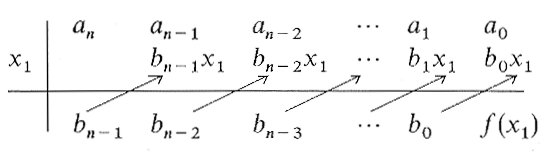
\includegraphics[width=6cm]{Content/Rechenregeln/hornerschema_1.png}\\
		$x_1 \Rightarrow$ Nullstelle (muss erraten werden!!)\\
		oberste Zeile = zu zerlegendes Polynom			
	\end{minipage}
	\begin{minipage}[t]{9cm}
		\textbf{Beispiel:}\\
		$f(x) = x^3-67x-126$\\
		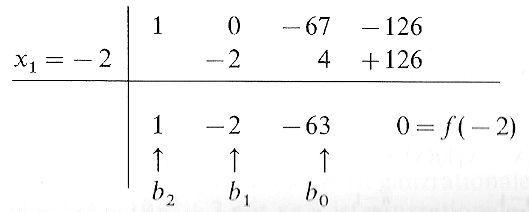
\includegraphics[width=6cm]{Content/Rechenregeln/hornerschema_2.png}\\
		$\Rightarrow f(x) = (x-x_1)(b_2x^2 + b_1x + b_0) = (x+2)(x^2-2x-63)$	
	\end{minipage}
			
	\subsection{Trigonometrie}
			$\sin^2(b)+\cos^2(b)=1 \qquad \tan(b)=\frac{\sin(b)}{\cos(b)} \qquad \cosh(b)^2 - \sinh(b)^2 = 1 \qquad \tanh(b)=\frac{\sinh(b)}{\cosh(b)}$
\subsubsection{Funktionswerte für Winkelargumente}
	\renewcommand{\arraystretch}{1.5}
	\begin{minipage}{5cm}
		\begin{tabular}[c]{ |c|c||c|c|c| }
	    	\hline
			deg & rad & sin & cos & tan\\
			\hline
			0\symbol{23} & 0 & 0 & 1 & 0\\
			\hline
			30\symbol{23} & $\frac{\pi}{6}$ & $\frac{1}{2}$ & $\frac{\sqrt{3}}{2}$ &
			$\frac{\sqrt{3}}{3}$\\
			\hline
			45\symbol{23} & $\frac{\pi}{4}$ & $\frac{\sqrt{2}}{2}$ & $\frac{\sqrt{2}}{2}$
			& 1\\
			\hline
			60\symbol{23} & $\frac{\pi}{3}$ & $\frac{\sqrt{3}}{2}$ & $\frac{1}{2}$ &
			$\sqrt{3}$\\
			\hline			
		\end{tabular}			
	\end{minipage}
	\begin{minipage}{4.3cm}
		\begin{tabular}[c]{ |c|c||c|c|}
	    	\hline
			deg & rad & sin & cos\\
			\hline
			90\symbol{23} & $\frac{\pi}{2}$ & 1 & 0\\
			\hline	
			120\symbol{23} & $\frac{2\pi}{3}$ & $\frac{\sqrt{3}}{2}$ & $-\frac{1}{2}$ \\
			\hline
			135\symbol{23} & $\frac{3\pi}{4}$ & $\frac{\sqrt{2}}{2}$ & $-\frac{\sqrt{2}}{2}$\\
			\hline
			150\symbol{23} & $\frac{5\pi}{6}$ & $\frac{1}{2}$ & $-\frac{\sqrt{3}}{2}$\\
			\hline
		\end{tabular}			
	\end{minipage}
	\begin{minipage}{4.5cm}
		\begin{tabular}[c]{ |c|c||c|c| }
	    	\hline
			deg & rad & sin & cos\\
			\hline
			180\symbol{23} & $\pi$ & 0 & -1\\
			\hline	
			210\symbol{23} & $\frac{7\pi}{6}$ & $-\frac{1}{2}$ & $-\frac{\sqrt{3}}{2}$\\
			\hline
			225\symbol{23} & $\frac{5\pi}{4}$ & $-\frac{\sqrt{2}}{2}$ & $-\frac{\sqrt{2}}{2}$\\
			\hline
			240\symbol{23} & $\frac{4\pi}{3}$ & $-\frac{\sqrt{3}}{2}$ & $-\frac{1}{2}$\\
			\hline
		\end{tabular}			
	\end{minipage}
	\begin{minipage}{4.5cm}
		\begin{tabular}[c]{ |c|c||c|c| }
	    	\hline
			deg & rad & sin & cos\\
			\hline
			270\symbol{23} & $\frac{3\pi}{2}$ & -1 & 0\\
			\hline	
			300\symbol{23} & $\frac{5\pi}{3}$ & $-\frac{\sqrt{3}}{2}$ & $\frac{1}{2}$\\
			\hline
			315\symbol{23} & $\frac{7\pi}{4}$ & $-\frac{\sqrt{2}}{2}$ & $\frac{\sqrt{2}}{2}$\\
			\hline
			330\symbol{23} & $\frac{11\pi}{6}$ & $-\frac{1}{2}$ & $\frac{\sqrt{3}}{2}$\\
			\hline
		\end{tabular}			
	\end{minipage}
	\renewcommand{\arraystretch}{1}
	
\subsubsection{Quadrantenbeziehungen}
	\begin{tabbing}
    	xxxxxxxxxxxxxxxxxxxxxxxxxxxxxxxxxx \= \kill
	  	$\sin(-a)=-\sin(a)$ \> $\cos(-a)=\cos(a)$\\
		$\sin(\pi - a)=\sin(a)$ \> $\cos(\pi - a)=-\cos(a)$\\
		$\sin(\pi + a)=-\sin(a)$ \> $\cos(\pi +a)=-\cos(a)$\\
		$\sin\left(\frac{\pi}{2}-a \right)=\sin\left(\frac{\pi}{2}+a \right)=\cos(a)$ \>
		$\cos\left(\frac{\pi}{2}-a \right)=-\cos\left(\frac{\pi}{2}+a \right)=\sin(a)$  
    \end{tabbing}

	\textbf{Additionstheoreme}
		$\sin(a \pm b)=\sin(a) \cdot \cos(b) \pm \cos(a) \cdot \sin(b) \qquad
		\cos(a \pm b)=\cos(a) \cdot \cos(b) \mp \sin(a) \cdot \sin(b)$\\ 
		$\tan(a \pm b)=\dfrac{\tan(a) \pm \tan(b)}{1 \mp \tan(a) \cdot \tan(b)}$
		
	\subsubsection{Doppel- und Halbwinkel}	
		\begin{tabular}{ll}
			$\sin(2a)=2\sin(a)\cos(a)$ &
			$\cos(2a)=\cos^2(a)-\sin^2(a)=2\cos^2(a)-1=1-2\sin^2(a)$\\
			$\cos^2 \left(\frac{a}{2}\right)=\frac{1+\cos(a)}{2}$ &
			$\sin^2 \left(\dfrac{a}{2}\right)=\frac{1-\cos(a)}{2}$
		\end{tabular}\\
		
	\begin{minipage}[t]{9.5cm}	
		\subsubsection{Produkte}
			$\sin(a)\sin(b)=\frac{1}{2}(\cos(a-b)-\cos(a+b))$\\
			$\cos(a)\cos(b)=\frac{1}{2}(\cos(a-b)+\cos(a+b))$\\
			$\sin(a)\cos(b)=\frac{1}{2}(\sin(a-b)+\sin(a+b))$
		\subsubsection{Hyperbolic}
			$\sinh(z) = \frac{1}{2} \left( e^z - e^{-z} \right) \qquad \cosh(z) =
			\frac{1}{2} \left( e^z + e^{-z} \right) $
	\end{minipage}
	\hfill
	\begin{minipage}[t]{9.5cm}		
		\subsubsection{Summe und Differenz}
			$\sin(a)+\sin(b)=2 \cdot \sin \left(\frac{a+b}{2}\right) \cdot
			\cos\left(\frac{a-b}{2}\right)$\\
			$\sin(a)-\sin(b)=2 \cdot \sin \left(\frac{a-b}{2}\right) \cdot
			\cos\left(\frac{a+b}{2}\right)$\\
			$\cos(a)+\cos(b)=2 \cdot \cos \left(\frac{a+b}{2}\right) \cdot
			\cos\left(\frac{a-b}{2}\right)$\\
			$\cos(a)-\cos(b)=-2 \cdot \sin \left(\frac{a+b}{2}\right) \cdot
			\sin\left(\frac{a-b}{2}\right)$\\
			$\tan(a) \pm \tan(b)=\dfrac{\sin(a \pm b)}{\cos(a)\cos(b)}$
	\end{minipage}	
	
		
	\subsubsection{Euler}
	$sin(z)=\frac{e^{jz}-e^{-jz}}{2j} \hspace{2cm}
    cos(z)=\frac{e^{jz}+e^{-jz}}{2} \hspace{2cm}
    e^{j\varphi}=cjs(\varphi)=cos(\varphi)+j sin(\varphi)$
    
    \subsubsection{Komplex}
    \begin{tabular}{lll}
     	Betrag: & $ |z| = \sqrt{Re(z)^2 + Im(z)^2} = \sqrt{z \cdot \bar{z}}$\\ 
     	Konjugiertkomplex: & $z=z_1 + jz_2$ & $\bar{z}=z^*=z_1-jz_2$
     \end{tabular}
	
			
	\subsection{Taylor Polynom}
		$f(x_0+h)=f(x_0) + f'(x_0)h + \frac{f''(x_0)}{2}h^2 + \frac{f'''(x_0)}{3!}h^3 + \ldots + \frac{f^{(n)}(x_0)}{n!}h^n + R_n(x_0, h)$

	\subsection{Integralrechnung}	
	\begin{tabbing}
	     xxxxxxxxxxxxxxxxxxxxxxxxxxxxxxx \= xxx \= xxxxxxxxxxxxxxxxxxxxxxxxxxxxxxxxxxxxxxxxxxxxxxxxxxxxxxx\kill  
	     Integration\>\>$A=\int\limits_{a}^{b}{f(t)dt}=\left[F(t)\right]_a^b=F(b)-F(a)$\\[0.2cm]
	     Linearität\>		  
	   $\qquad\int{f(\alpha x+\beta )dx=\frac{1}{\alpha}\cdot F(\alpha x+
				\beta)+C}$\\[0.2cm]
		   Partielle Integration\>
	   $\qquad\int\limits_a^b{\underset{\Uparrow}{u}'(x)\cdot \underset{\Downarrow}{v}(x)dx}=\biggl[ u(x)\cdot v(x) \biggr]_a^b
	   -\int\limits_a^b{u(x)\cdot v'(x)dx}$\\[0.2cm]
	   Substitution (Rationalisierung)\>
	   $\qquad t=\tan\frac{x}{2}, \qquad dx=\frac{2dt}{1+t^2} \qquad 
	   \sin  x=\frac{2t}{1+t^2} \qquad \cos x=\frac{1-t^2}{1+t^2}
				\quad\int{R(\sin(x)\cos(x))dx}$\\ 
	   Allgemeine Substitution \> \>
				$\int\limits_{a}^{b}{f(x)dx}=\int\limits_{g^{-1}(a)}^{g^{-1}(b)}{f(g(t))\cdot
				g'(t)dt}\qquad t=g^{-1}(x)\qquad  \fbox{x=g(t)}\qquad dx=g'(t)\cdot dt$\\
	   Logarithmische Integration \>\>
	    $ \int{\frac{f'(x)}{f(x)}dx}=\ln|f(x)|+C	\qquad{(f(x)\neq 1)}$\\[0.2cm]
	  Spezielle Form des Integranden \>\>
		 		$\int{f'(x)\cdot (f(x))^{\alpha} dx}= f(x)^{\alpha +1}\cdot
		 		\frac{1}{\alpha+1}+C \qquad{(\alpha \neq -1)}$\\ 
	   Differentiation\>\>
		 		$\int \limits ^{b} _{a} {f'(t)dt}=f(b)-f(a)$\qquad
				$\frac{d}{dx} \int \limits ^{x} _{1} {f(t)dt}=f(x)$
	\end{tabbing}
	%\subsubsection{Einige unbestimmte Integrale}
	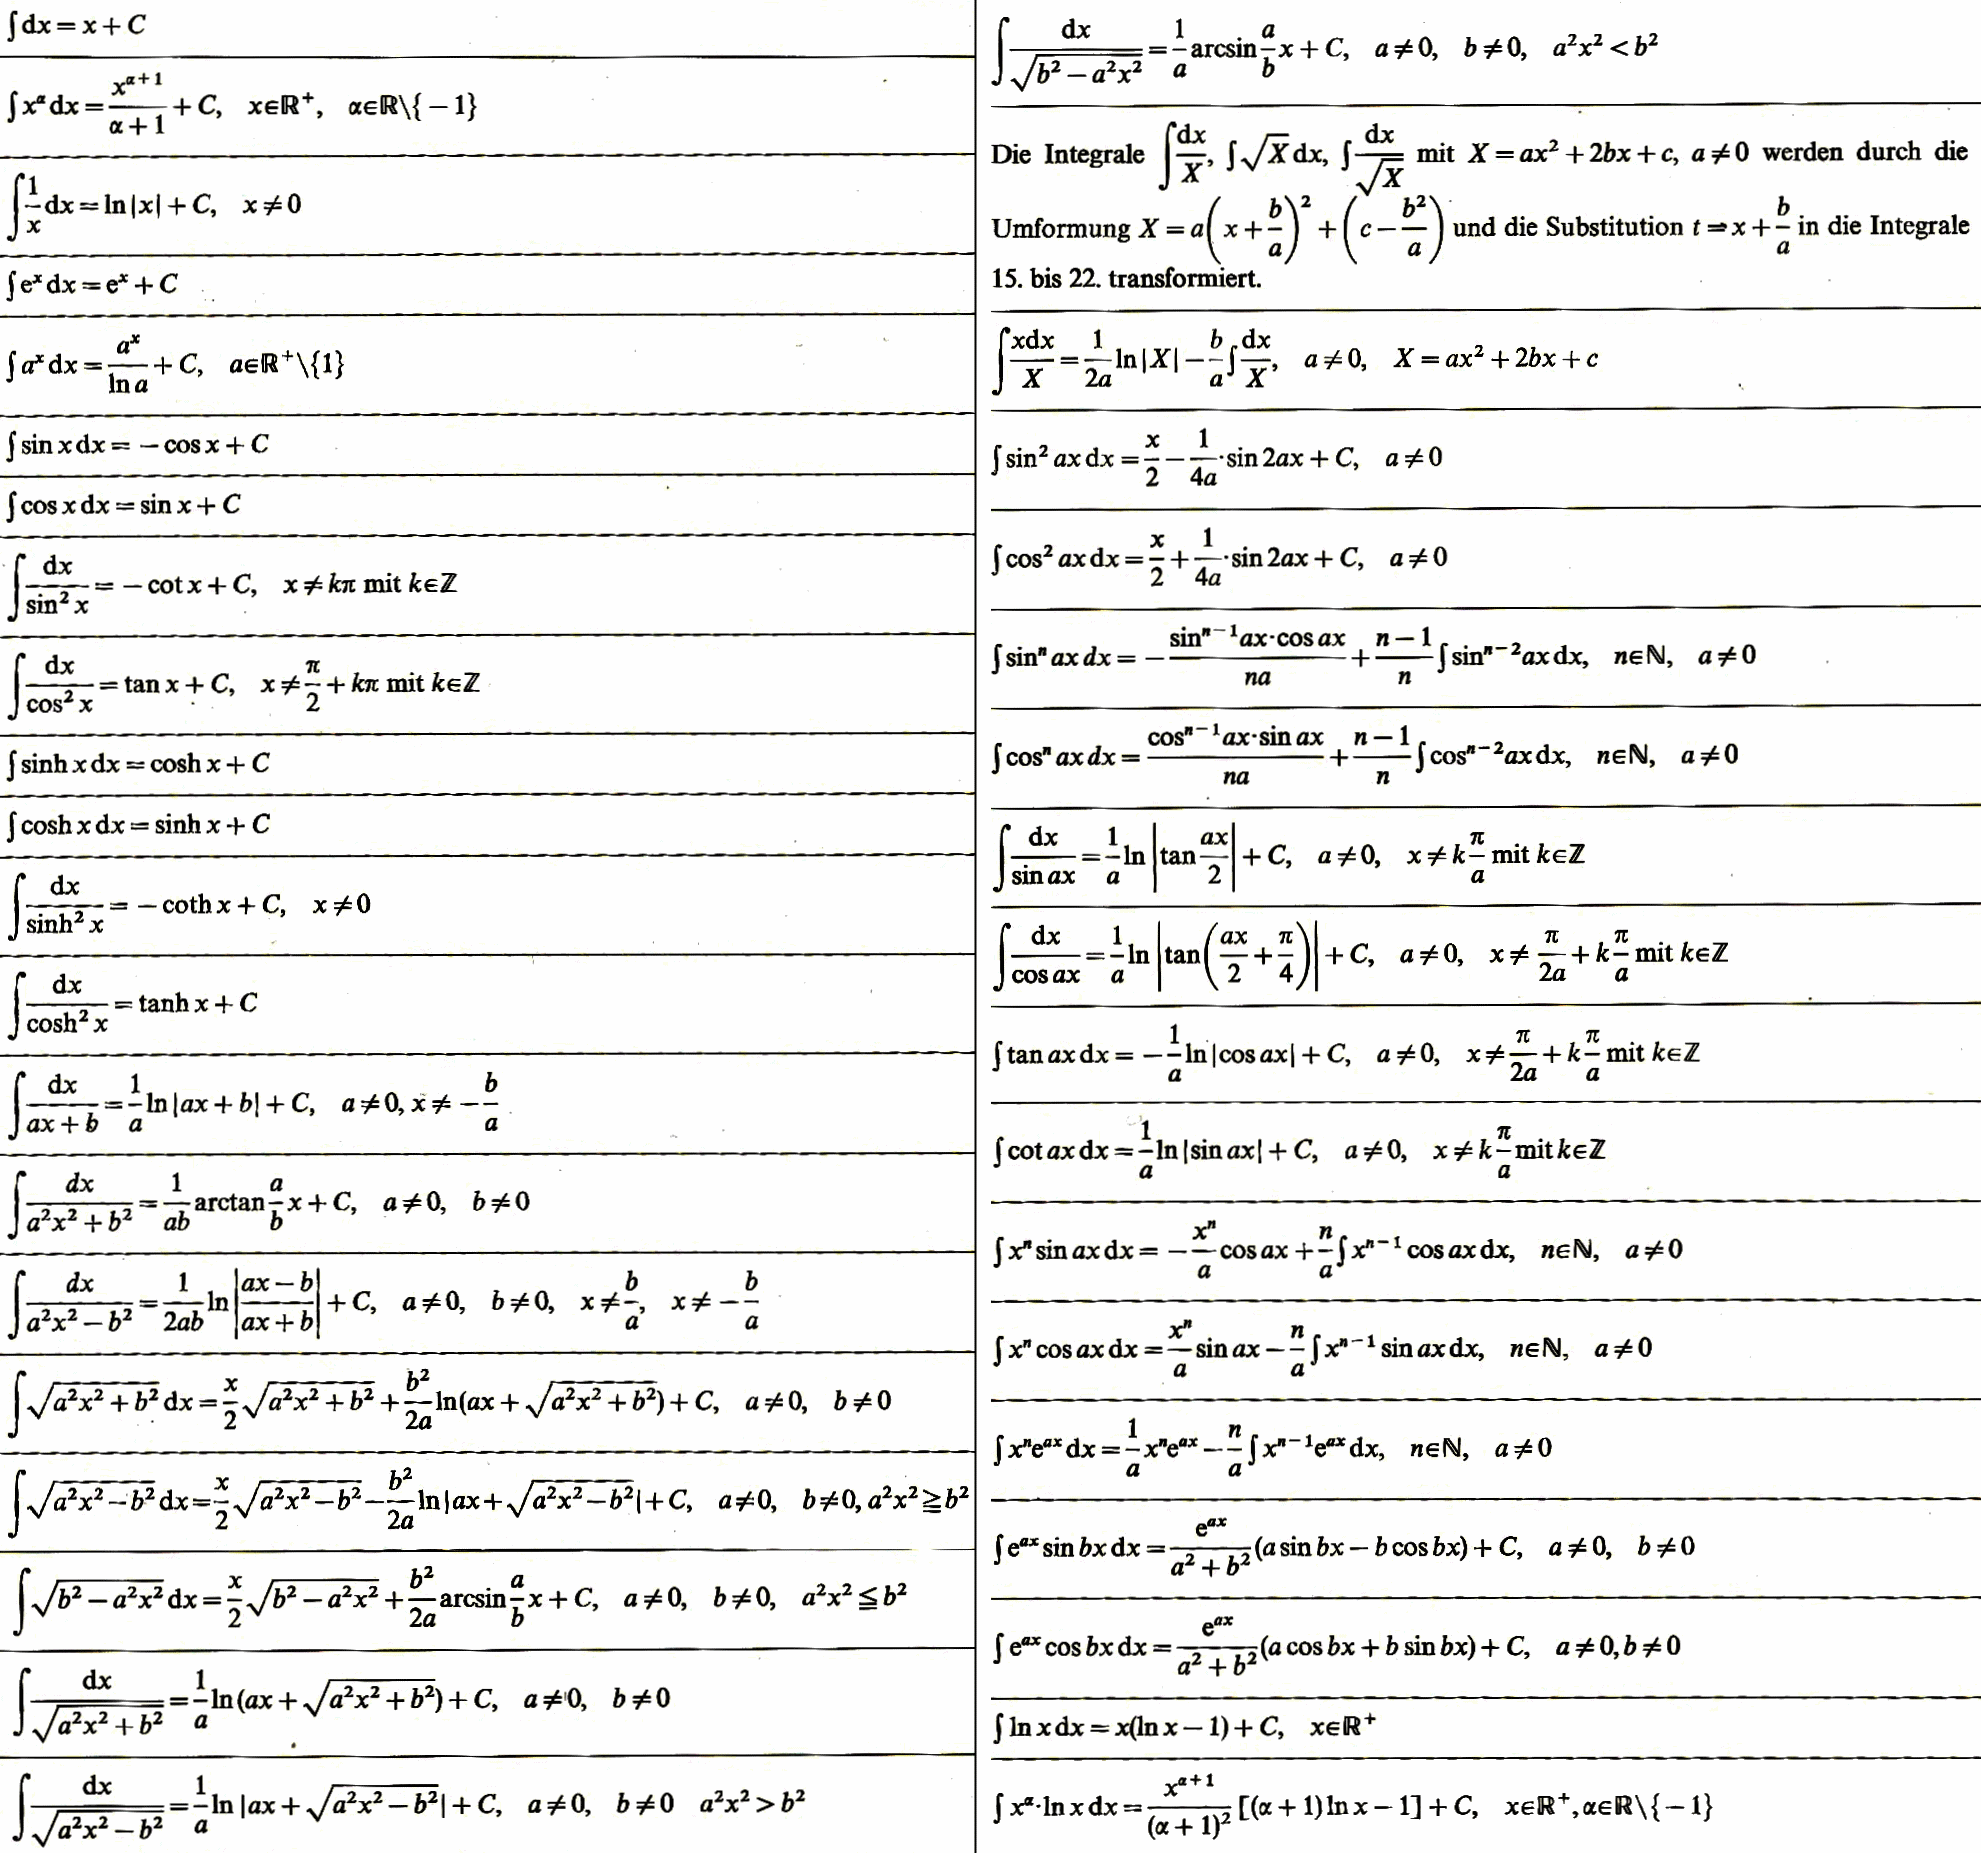
\includegraphics[width=19cm]{Content/Rechenregeln/integrale.png} 
	
	$\int \mathrm dx = x + C$\\
	$\int x^{\alpha} \mathrm dx = \frac{x^{\alpha + 1}}{\alpha + 1} + C$, $x \in
	\mathbb{R}^+$, $\alpha \in \mathbb{R} \textbackslash \{-1\}$\\
	$\int \frac{1}{x} \mathrm dx = ln \lvert x \lvert + C$, $x \neq 0$\\
	$\int e^x \mathrm dx = e^x + C$\\
	$\int a^x \mathrm dx = \frac{a^x}{ln(a)} + C$, $a \in \mathbb{R}^+
	\textbackslash \{1\}$\\
	$\int sin x \mathrm dx = - cos x + C$\\
	$\int cos x \mathrm dx = sin x + C$\\
	$\int \frac{\mathrm dx}{sin^2 x} = -cot(x) + C$, $x \neq k \pi$ mit $k \in
	\mathbb{Z}$\\
	$\int \frac{\mathrm dx}{cos^2 x} = tan(x) + C$, $x \neq \frac{\pi}{2} + k \pi$
	mit $k \in \mathbb{Z}$\\
	$\int sinh(x) \mathrm{dx} = cosh(x) + C$\\
	$\int cosh(x) \mathrm{dx} = sinh(x) + C$\\
	$\int \frac{\mathrm dx}{sinh^2 x} = -coth(x) + C$, $x \neq 0$\\
	$\int \frac{\mathrm dx}{cosh^2 x} = tanh(x) + C$, $x \neq 0$\\
	$\int \frac{\mathrm dx}{ax + b} = \frac{1}{a} ln \lvert ax + b \lvert + C$, $a
	\neq 0$, $x \neq - \frac{b}{a}$\\
	$\int \frac{\mathrm dx}{a^2x^2 + b^2} = \frac{1}{ab} arctan(\frac{a}{b} x) +
	C$, $a \neq 0$, $x \neq - \frac{b}{a}$ $x \neq -\frac{b}{a}$\\
	$\int \frac{\mathrm dx}{a^2x^2 - b^2} = \frac{1}{2ab} ln \lvert \frac{ax -
	b}{ax + b} \lvert + C$, $a \neq 0$, $x \neq - \frac{b}{a}$ $x \neq
	-\frac{b}{a}$\\
	$\int \sqrt{a^2 x^2 + b^2} \mathrm dx = \frac{x}{2} \sqrt{a^2 x^2 + b^2} +
	\frac{b^2}{2a} ln(ax + \sqrt{a^2 x^2 + b^2}) + C$, $a \neq 0$, $b \neq 0$\\
	$\int \sqrt{a^2 x^2 - b^2} \mathrm dx = \frac{x}{2} \sqrt{a^2 x^2 - b^2} +
	\frac{b^2}{2a} ln \lvert ax + \sqrt{a^2 x^2 - b^2} \lvert + C$, $a \neq 0$, $b
	\neq 0$, $a^2 x^2 \geq b^2$\\
	$\int \sqrt{b^2 - a^2x^2} \mathrm dx = \frac{x}{2} \sqrt{b^2 - a^2x^2} +
	\frac{b^2}{2a} arcsin(\frac{a}{b} x) + C)$, $a \neq 0$, $b \neq 0$,
	$a^2 x^2 \geq b^2$\\
	$\int \frac{\mathrm dx}{\sqrt{a^2 x^2 + b^2}} = \frac{1}{a} ln(ax +
	\sqrt{a^2 x^2 + b^2}) + C$, $a \neq 0$, $b \neq 0$\\
	$\int \frac{\mathrm dx}{\sqrt{a^2 x^2 - b^2}} = \frac{1}{a} ln(ax +
	\sqrt{a^2 x^2 - b^2}) + C$, $a \neq 0$, $b \neq 0$ $a^2 x^2 > b^2$\\
			
	\subsection{Differentialgleichungen}
			\subsubsection{Lineare Differentialgleichungen 1. Ordnung}
	\begin{tabular}{lll}
	\textbf{Form:} $ y'+f(x)y = g(x) $ &
	\textbf{Vorgehen:} $y=y_H+y_p$ &
	$y_H=k \cdot e^{-\int f(x) dx}$ wobei $k=y_0$\\ & &
	$y_p=k \cdot e^{-\int f(x) dx}$ wobei $k=\int(g(x) \cdot e^{\int f(x) dx}) dx$
	\end{tabular}
	
	\subsubsection{Lineare Differentialgleichung 2. Ordnung mit konstanten 
	Koeffizienten}
	\begin{tabular}{p{8cm}p{8cm}}
	\textbf{Form:} $y''+a_1\cdot y'+a_0\cdot y=f(x)$  &
	\textbf{St"orglied:} $f(x)$\\
	\textbf{Homogene Differentialgleichung:} $f(x)=0$ &
	\textbf{Inhomogene Differentialgleichung:} $f(x)\neq 0$
	\end{tabular}
	
	\subsubsection{Allgemeine Lösung einer homogenen DGL:\quad\subsubadd{$\quad
	Y_H$}}
	\textbf{Charakteristisches Polynom}
	$\qquad\underline{\lambda^2+a_1\cdot\lambda+a_0=0}$ \hspace{1cm}von
	$\qquad\underline{y''+a_1\cdot y'+a_0\cdot y=0}$ 
	$\qquad(\lambda_{1,2} = -\frac{a_1}{2} \pm \frac{\sqrt{a_1^2 - 4a_0}}{2})$\\ \\
	\begin{tabular}{p{8cm}p{8cm}}
	Falls $\lambda_1\neq \lambda_2$ und $\lambda_{1,2} \in R$:&
	$Y_H=Ae^{\lambda_1x}+Be^{\lambda_2x}$\\
	Falls $\lambda_1=\lambda_2$ und $\lambda_{1,2} \in R$:    &
	$Y_H=e^{\lambda_1x}(A+B\cdot x)$\\
	Falls $\lambda_{1,2}=-\frac{a_1}{2}\pm j\alpha$:          &
	$Y_H=e^{-\frac{1}{2}a_1x}(Acos(\alpha x) +Bsin(\alpha x))$\\
	\end{tabular}\\
	
	\subsubsection{Allgemeine L"osung einer inhomogenen DGL:\quad\subsubadd{$y=Y_H+y_P$}}
	
	\textbf{Grundl"oseverfahren einer inhomogenen DGL:\quad\subsubadd{$\quad y_P$}}\\
	Homogene DGL: $y''+a_1\cdot y'+a_0\cdot y=0$  f"ur die ($g(x)=Y_H$ homogene Loesung)  $g(x_0)=0$  und
	$g'(x_0)=1$  gilt, ist:\\
	$$y_P(x)=\int\limits_{x_o}^{x} g(x+x_0-t)\cdot f(t)dt$$\\
	die partikul"are L"osung von $y''+a_1\cdot y'+a_0\cdot y=f(x)$\\
	
	\textbf{Der Ansatz einer inh. DGL in Form des
	St"orgliedes:\quad\subsubadd{$\quad y_P$}}\\
	
	 $f(x)=p_n(x)$\hspace{9cm}($p_n(x)$
	und $q_n(x)$ sind Polynome vom gleichen Grad)\\
	\begin{tabular}{p{8cm}p{4cm}}
	Fall a: $a_0\neq 0$:          & $y_P = q_n(x)$\\
	Fall b: $a_0 = 0 , a_1\neq 0$:& $y_P=x\cdot q_n(x)$\\
	Fall c: $a_0=a_1=0$:          & $y_P=x^2\cdot q_n(x)$\\
	\end{tabular}\\
	\\
	
	$f(x)=e^{bx}\cdot p_n(x)$\\
	\begin{tabular}{p{8cm}p{4cm}}
	Fall a: $b$ nicht Nullstelle des char. Polynoms:    &
	$y_P=e^{bx}\cdot q_n(x)$\\
	Fall b: $b$ einfache Nullstelle des char. Polynoms: &
	$y_P=e^{bx}\cdot x \cdot q_n(x)$\\
	Fall c: $b$ zweifache Nullstelle des char. Polynoms:&
	$y_P=e^{bx}\cdot x^2\cdot q_n(x)$\\
	\end{tabular}\\
	\\
	
	$f(x)=e^{cx}\cdot (p_n(x)\cos(bx)+q_n(x)\sin(bx))$\\
	\begin{tabular}{p{8cm}p{8cm}}
	Fall a: $c+jb$ nicht Loesung der char. Gleichung:    &
	$y_P=e^{cx}\cdot (r_n(x)\cos(bx)+s_n(x)\sin(bx))$\\
	Fall b: $c+jb$ Loesung der char. Gleichung: &
	$y_P=e^{cx}\cdot x\cdot(r_n(x)\cos(bx)+s_n(x)\sin(bx))$\\
	\end{tabular}\\
	\\

	\textbf{Superpositionsprinzip}
	
	$f(x)=c_1f_1(x)+c_2f_2(x)$\\
	\begin{tabular}{p{8cm}p{4cm}}
	$y_1$ ist spezielle L"osung der DGL &
	$y''+a_1\cdot y'+a_0\cdot y=c_1f_1(x)$ \\
	$y_2$ ist spezielle L"osung der DGL &
	$y''+a_1\cdot y'+a_0\cdot y=c_2f_2(x)$ \\
	dann ist:                          &
	$y_P=c_1y_1+c_2y_2$\\
	\end{tabular}
	
	\newpage
	
	\subsubsection{Lineare Differentialgleichung n. Ordnung mit konstanten Koeffizienten}
	\begin{tabular}{p{4cm}p{12cm}}
	\textbf{Form:} &
	$y^{(n)}+a_{n-1}\cdot y^{(n-1)}+\ldots +a_0\cdot y=f(x)$ $\Leftrightarrow$ $\sum\limits_{k=0}^na_ky^{(k)}=f(x)$\\
	\end{tabular}
	
	\textbf{Homogene L"osungen}\\
	\begin{tabular}{lll}
	Fall a: r reelle L"osungen $\lambda$: 
		& $y_1=e^{\lambda x}$, $y_2=xe^{\lambda x}$, \ldots
		,$y_r=x^{r-1}e^{\lambda x}$ 
		& Starke D"ampfung/Kriechfall\\
	Fall b: $k$ komplexe L"osungen $\lambda=\alpha +j\beta$: 
		&$y_1=e^{\alpha x}\cos(\beta x)$, $y_{3}=e^{\alpha x}x^1\cos(\beta
	x),...$ (ungerade)
		& Schwache D"ampfung /\\
		&$y_{2}=e^{\alpha x}\sin(\beta x)$, $y_{4}=e^{\alpha
	x}x^{1}\sin(\beta x),...$ (gerade)
		& Schwingfall\\
	\end{tabular}
	
	Freiheitsgrade $(A,B,C, ...)$ und zusaetzliches $x^{n}$ nicht vergessen!!! 
	
	\textbf{Allgemeinste L"osung des partikul"aren Teils:}\\
	$$\underbrace{\sum_{k=0}^n a_k y^{(k)}}_{f(y,y',y'',\ldots)} = \underbrace{e^{\alpha x} (p_{m1}(x) \cos (\beta x) + q_{m2}(x) \sin (\beta x))}_{\text{St"orglied}}$$
	Unterscheide die L"osungen des charakteristischen Polynoms ($\lambda$):\hspace{5.5cm}mit m = max(m1, m2)\\
	\begin{tabular}{p{8cm}p{8.5cm}}
	Fall a: $\alpha + j\beta \neq \lambda$, so ist &
	$y_P = e^{\alpha x}(r_m(x)\cos(\beta x) + s_m(x) \sin(\beta x))$\\
	Fall b: $\alpha + j\beta$  ist u-fache L"osung von $\lambda$, so ist &
	$y_P = e^{\alpha x} x^u (r_m(x) \cos(\beta x) + s_m(x) \sin(\beta x))$\\
	&
	u-fache Resonanz
	
	\end{tabular}
	
	\textbf{Grundl"oseverfahren}\\
	\begin{tabular}{p{12cm}p{5cm}}
	$\begin{pmatrix}
	g(x_0)=  & 0 & = & c_1g_1(x_0)+c_2g_2(x_0)+\ldots +c_n(x_0)\\
	g'(x_0)= & 0 & = & c_1g_1'(x_0)+c_2g_2'(x_0)+\ldots +c_ng_n'(x_0)\\
	\vdots  & \vdots & \\                            
	g^{(n-1)}(x_0)= & 1 & = & c_1g_1^{(n-1)}(x_0)+c_2g_2^{(n-1)}(x_0)+\ldots
	+c_ng_n^{(n-1)}(x_0)
	\end{pmatrix}$ &
	\begin{minipage}[t]{5cm}
	ergibt $c_1,\ldots ,c_n$ f"ur\\
	$y_{P}(x)=\int_{x_0}^x{g(x+x_0-t)f(t)dt}$
	\end{minipage}
	\end{tabular}
	
	
	\subsubsection{Lineare Differentialgleichungssysteme erster Ordnung mit konstanten
	Koeffizienten}
	\begin{tabular}{p{8cm}p{8cm}}
	\textbf{Form:}&
	$\dot{x}=ax+by+f(t) \leftrightarrow y=\frac{1}{b}(\dot{x}-ax-f(t))$\\
	&
	$\dot{y}=cx+dy+g(t)$\\
	\textbf{Die allgem. L"osung ergibt sich aus der DGL:}&
	$\ddot{x}-(a+d)\dot{x}+(ad-bc)x=\dot{f}(t)-d \cdot f(t)+b \cdot g(t)$\\
	\end{tabular}
	
	$\ddot{x}, \dot{x}, \dot{y}$ sind jeweils nach $t$ abgeleitet!
	
	\subsubsection{DGL mit Laplacetransformation L"osen}
		Um eine DGL mit Laplace(kausal!) zu l"osen muss die gleichung zuerst in den
		Bildbereich transformiert werden. Nachher kann die gleichung Algebraisch
		gel"ost werden. Das Resultat muss dann "uber die R"ucktransformation wieder in
		den Orginalbereich transformiert werden.  \\
	
		Bemerkung:\\
		- $H(s)=\frac{1}{p(s)}$ wobei $p(s)$ das charakteristische Polynom darstellt

		\textbf{Stabilit"at}\\
			Ein System ist Stabil wenn die Nullstelle vom charakteristischen Polynom
			$p(s)$ in der Linken Halbebene zuliegen kommt:\\
			$$Re[p(s)] < 0$$
			
	\subsubsection{G"angige DGLs}
	  \label{sec:dgls}
	  \begin{tabular}{ll | ll}
	    DGL & L"osung & DGL & L"osung\\[0.2cm]
      $\dfrac{dx}{dt} =0$
      & $x_0$
 	    & $\dfrac{dx}{dt} =1$
 	    & $t + x_0$\\[0.2cm]
	    $\dfrac{dx}{dt} = y$
	    & $y \cdot t$
	    & $\dfrac{dx}{dt} = x$
	    & $C e^{t}$\\[0.2cm]
	    $\dfrac{d u}{dt} = \sin(u)$
	    & $- \cos(u)$
	    & $\dfrac{d^2 x}{dt^2} = x$
	    & $\sinh(t)$ oder $\cosh(t)$\\[0.2cm]
	    $\dfrac{d^2 x(t)}{dt^2} = -\omega^2 x(t)$
	    & $A \omega \cos(\omega t) - B \omega \sin(\omega t)$
	    & & 
	  \end{tabular}
	
	\subsection{Differential-Rechnung}
	  $f'(x_0)=\lim\limits_{\Delta x\rightarrow 0}
	  \frac{f(x_0+\Delta)x-f(x_0)}{\Delta x}$\\
		\begin{tabular}{llll}
			Kettenregel:	& $f\big(g(x)\big)$ &$=$ & $g'(x)\cdot f'\big(g(x)\big)$
			oder $\frac{d f(g(x))}{dx} = f'(g(x)) \cdot g'(x)$\\[0.1cm] Produktregel:	&
			$f(x)\cdot g(x)$ &$=$ & $f'(x)\cdot g(x) + f(x)\cdot g'(x)$\\[0.1cm] Quotientenregel:& $\frac{f(x)}{g(x)}$ &$=$ & $\frac{f'(x)g(x)-f(x)g'(x)}{g^2(x)}$\\
		\end{tabular}
		
	\subsection{Diverses}	
	\begin{minipage}[t]{9.5cm}
		\subsubsection{Quadratische Lösungsformel}
			$ax^2+bx+c=0\quad\Rightarrow\quad x_{1,2}=\frac{-b\pm\sqrt{b^2-4ac}}{2a}$
	\end{minipage}
	\hfill
	\begin{minipage}[t]{9.5cm}
		\subsubsection{Determinanten}
			$\det\left(
			\begin{bmatrix}
				a_{11}&a_{12}\\
				a_{21}&a_{22}\\
			\end{bmatrix}\right)=
			\begin{vmatrix}
				a_{11}&a_{12}\\
				a_{21}&a_{22}\\
			\end{vmatrix}=a_{11}a_{22}-a_{12}a_{21}$
	\end{minipage}\\
	
	
	\begin{minipage}[t]{9.5cm}
		\subsubsection{Matrizeninversion}
			$A=\begin{bmatrix}
						a_{11}&a_{12}\\
						a_{21}&a_{22}\\
				\end{bmatrix}\quad\Rightarrow\quad
			A^{-1}=\frac{1}{det(A)}
			\begin{bmatrix}
				a_{22}&-a_{12}\\
				-a_{21}&a_{11}\\
			\end{bmatrix}$
	\end{minipage}
	\hfill
	\begin{minipage}[t]{9.5cm}
		\subsubsection{Eigenwerte/ Eigenvektoren}
			Eigenwert: $\det(A-\lambda I)\quad\Rightarrow\quad \lambda i$\\
			Eigenvektor: $(A-\lambda_i I)v=0\quad\Rightarrow\quad v_i\qquad(\text{Für jedes }\lambda_i)$\\
			Definition: $ A\cdot \underline{v} = \lambda \cdot \underline{v} $
	\end{minipage}
	
	
	\begin{minipage}[t]{9.5cm}
		\subsubsection{TI-89}
			\textbf{Gleichung für mehrere Werte}\\
			$(3x+y^2) \mid x=1 \text{ and } y=2 \to Resultat$\\
			\textbf{Matrizeneditor}
			\begin{itemize}
			  \item APPS / Data/Matrix Editor
			  \item New
			  \item Type: Matrix
			  \item Variable, Row, Column definieren
			  \item Werte eingeben
			\end{itemize}
			
			\textbf{Gespeicherte Variabeln löschen}
			\begin{itemize}
			\item Explorer: 2nd / VAR-LINK
			\item Variable anwählen
			\item löschen: DEL
			\item Löschen Bestätigen: ENTER
			\end{itemize}
			
	\end{minipage}
	


\end{document}
